\chapter{Seismology}\label{ch:seismology}
\section{Introduction}
\subsection{Key concepts}
\begin{itemize}
    \item What are the four types of seismic waves?  What particle motion do
    they induce?  What is the difference between a body and surface wave?

    \item What is stress? strain?  What are the differences between normal and
    shear stress/strain?  How does stress and strain relate to Hooke's law
    (material constants, e.g.\ $\sigma_{ii} = E \epsilon_{ii}$)?

    \item What is the seismic cycle?  How does it relate the magnitude to the
        frequency of earthquakes?

    \item How do the material constants relate to velocities of seismic waves?
    Why do we like Poisson's ratio so much (see first seismic practical key)?

    \item What are the three types of focal mechanisms for idealized
    earthquakes?  How do focal mechanisms relate to motion during an earthquake?
    to the stresses acting on a fault (pre-quake)?  How does it relate to
    regional tectonics?

    \item What other types of focal mechanisms are possible?  How can we use the
    focal mechanism to tell us about the source?

\end{itemize}

\subsection{Mathematical symbols and units}
\begin{table}[hbtp]
    \centering
    \caption{Definitions of symbols.}
    \label{tab:seismosym}
    \begin{tabular}{@{}cll@{}}
        \toprule
        \textbf{Symbol} &
        \textbf{Quantity} &
        \textbf{SI Unit} \\
        \midrule
        $t$             & time                          & second, \si{s} \\
        $x$, $y$, $z$   & distance                      & meter, \si{m} \\
        $\tau$          & period                        & \si{s} \\
        $f$             & frequency                     & hertz, \si{s^{-1}} \\
        $\omega$        & angular frequency ($\omega = 2 \pi f$) & \si{rad.s^{-1}} \\
        $\lambda$       & wavelength                    & \si{m} \\
        $k$             & wavenumber ($k = 2\pi \lambda^{-1}$) & \si{rad.m^{-1}} \\
        $\vb{u}$      & displacement field            & --- \\
        $F$             & force                         & newton, \si{N} \\
        $A$             & area                          & $m^2$ \\
        $\sigma$        & stress                        & pascal, $\si{Pa} = \si{N.m^{-2}}$ \\
        $\epsilon$      & strain                        & --- \\
        $\rho$          & density                       & \si{kg.m^{-3}} \\
        $\nu$           & Poisson's ratio               & --- \\
        $E$             & Young's modulus (tensile strength) & \si{Pa} \\
        $K$             & bulk modulus                  & \si{Pa} \\
        $\mu$           & shear modulus                 & \si{Pa} \\
        $V_P$, $\alpha$ & $P$-wave velocity             & \si{km.s^{-1}} \\
        $V_S$, $\beta$  & $S$-wave velocity             & \si{km.s^{-1}} \\
        \bottomrule
    \end{tabular}
\end{table}

\section{Seismology introduction}
{\it Seismology} is the study of elastic waves propagating through the Earth and
the most utilized method to study the internal structure of the planet. 

There will be two units discussed in these notes, passive source and active
source seismology.  While the underlying physical principles are the same, there
are some differences in processing and the unknowns.  {\it Passive source}
seismology is often called {\it earthquake seismology} or just seismology and
utilizes waves generated from a source with unknown location (space and time)
and characteristics (frequency range and radiation pattern).  Active source
seismology is often called {\it seismics} and utilizes a controlled source with
known location and characteristics.

The notes will start by covering the types of waves we expect to find within the
Earth and follow with the theory describing their formation and propagation.
Then we will cover a few topics of active and passive seismology.

\section{Seismic waves}
There are several types of seismic waves which propagate within the Earth, each
related to a specific type of particle motion and with differing velocities.
\begin{figure}[hbtp]
  \centerline{
    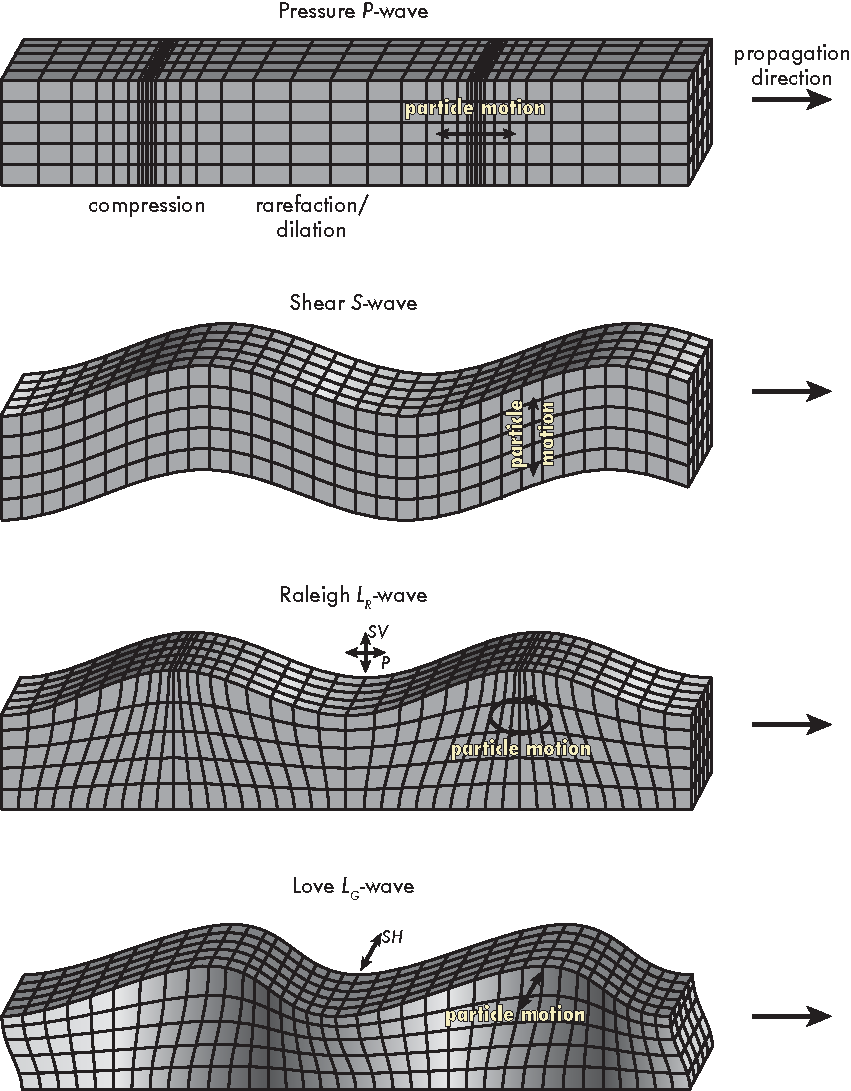
\includegraphics[]{seismology/figures/seismic_waves.pdf}
  }
  \caption{Types of seismic waves.  After Phillips (1968) and Bolt (1976).}
  \label{fig:waves}
\end{figure}


\subsection{Body waves}

\subsubsection{$P$-waves}
Also called compressional or pressure waves, $P$-waves are created by particle
motions in the direction parallel to the wave propagation.  $P$-waves can travel
through fluids such as the melts and air.  In fact the sound we hear is due to
this type of particle motion.


\subsubsection{$S$-waves}
Shear waves, $S$-waves, are created by particle motions that are orthogonal to
the direction of wave propagation.  We define two types of shear waves, $SH$ and
$SV$, to describe the $S$-waves propagating in the vertical and horizontal
direction.  $S$-waves cannot travel through fluids as fluids cannot support
shear motions, $\mu = 0$.

\subsection{Surface waves}
Surface waves are $P$- and $S$-waves that are captured at the free surface of the
Earth.  In a way, these waves are trapped.  The two types of surface waves are:
Raleigh waves, which includes both $P$- and $SV$-wave components where particle
travel in a circular motion; and Love waves, which include $SH$-wave components
where the particles move horizontally at the surface perpendicular to the
direction of propagation.

Most of the damage done due to Earthquakes is a result of surface waves.
Surface waves also travel at lower velocities than $P$-, and $S$-waves.  For
earthquakes at great distances away, it can be minutes between the arrival time
the first $P$-wave and subsequent surface waves.  Although the long delay surface
wave arrival is also related to the greater path length along the surface rather
than through the Earth.


\section{Stress and strain}
Before we can discuss wave propagation, we need to know why and how waves
propagate in the first place.  To do this, we need to understand how a material
behaves under stress.

{\it Stress} is the force applied per unit area and has the dimensions of
pressure, SI: Pa = N~m$^{2}$ (Figure~\ref{fig:ss}).

{\it Strain} represents the deformation of a body under an applied stress and
can be simply written as the change in distance between adjacent points in a
body as a function of their initial separation.  Strain is a unitless quantity
(Figure~\ref{fig:ss}).
\begin{figure}[hbtp]
  \centerline{
    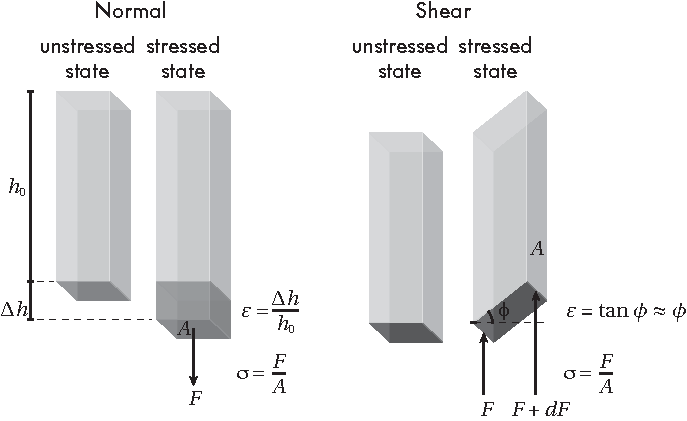
\includegraphics[]{seismology/figures/stress&strain.pdf}
  }
  \caption{Stress and strain under an applied normal and shear stress.}
  \label{fig:ss}
\end{figure}

The strain occurs as a result of applied stress.  The strain (deformation) may
be temporary, occurring under stress and restoring to the initial dimensions when
the stress is relieved, or semi-permanent to permanent, with partial or no
restoration of dimensions when stress is relieved.  When the former occurs, the
material is said to behave elastically.  When the latter occurs, the material is
said to behave plastically.  In general seismic waves propagate elastically
through the medium.

Figure~\ref{fig:hooke} shows the relationship between stress and
strain.  When the applied stress is low, the stress and strain can be related
linearly such that
\begin{equation*}
    \sigma = \frac{F}{A} \propto \frac{\Delta h}{h_0} = \epsilon.
\end{equation*}
This linear relationship is called Hooke's law and was originally used to
describe the behavior springs.  The linear proportionality breaks down as
greater stress is applied.  The deformation may still be fully restorable in
this case up to the elastic limit.  This region is called anelastic deformation.
Deformation at stresses beyond the elastic limit are said to plastically deform
and may be partially restorable.
\begin{figure}[hbtp]
  \centerline{
    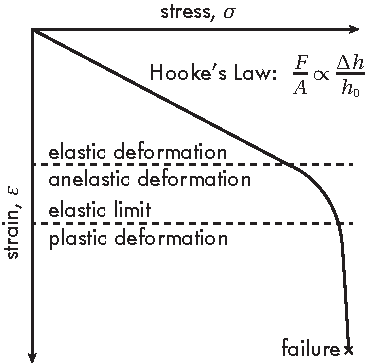
\includegraphics[]{seismology/figures/hookes_law.pdf}
  }
  \caption{The relationship between stress and strain.  Hooke's law is only
  valid in the range where strain linearly responds to stress.  After
  \citet{Lowrie1997}.}
  \label{fig:hooke}
\end{figure}


\subsection{Stress, $\sigma$}
In simplest terms, the stress is defined as
\begin{equation}
    \sigma_{ij} = \lim_{A_j \to 0} \frac{F_i}{A_j}
\end{equation}
where the subscript $i$ refers to the axis parallel to the applied force and the
subscript $j$ refers to the axis normal to the area upon which the force is
applied.

There are two types of stress: normal stress, applied force perpendicular to a
planar area (i.e.\ $i = j$); and shear stress, applied force parallel to a
planar area (i.e. $i \neq j$).  Hence for forces applied to $A_x$, we have the
three possible stress combinations
\begin{align*}
    \sigma_{xx} = & \lim_{A_x \to 0} \frac{F_x}{A_x} &\quad \text{normal stress} \\
    \sigma_{yx} = & \lim_{A_x \to 0} \frac{F_y}{A_x} &\quad \text{shear stress} \\
    \sigma_{zx} = & \lim_{A_x \to 0} \frac{F_z}{A_x} &\quad \text{shear stress}
\end{align*}
Consider some cubic volume element of some solid (infinitesimally small), there
are three axes upon which forces may be applied to each face of the cube
(Figure~\ref{fig:stress}).  Accounting for each normal and shear stress, there
are 9 possible combinations of forces applied to the faces which we can write in
matrix form as
\begin{equation*}
    \vb{\sigma} =
    \begin{bmatrix}
        \sigma_{xx} & \sigma_{xy} & \sigma_{xz} \\
        \sigma_{yx} & \sigma_{yy} & \sigma_{yz} \\
        \sigma_{zx} & \sigma_{zy} & \sigma_{zz}
    \end{bmatrix}.
\end{equation*}
This matrix is called the stress tensor.  If there is no net rotation of the
body then $\sigma_{ij} = \sigma_{ji}$ for $i \neq j$, which allows us to
simplify the matrix to six independent quantities.
\begin{figure}[hbtp]
  \centerline{
    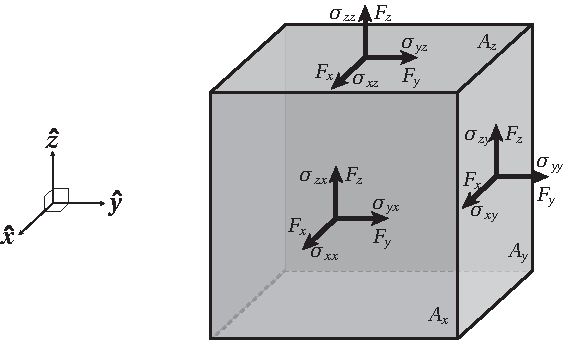
\includegraphics[]{seismology/figures/stress_element.pdf}
  }
  \caption{Stress on faces of a cube.}
  \label{fig:stress}
\end{figure}


\subsection{Strain, $\epsilon$}
Just as there are two types of stress (normal and shear), there are two types of
strain (dilation and shear).  Unlike stress which is simply the force times the
area, the strain between the dilation and shear must be treated separately.

{\bf Normal or longitudinal strain} is strain that occurs normal to the faces of
a discrete element,
\begin{align}
    \epsilon_{xx} & = \pdv{u_x}{x} \\
    \epsilon_{yy} & = \pdv{u_y}{y} \\
    \epsilon_{zz} & = \pdv{u_z}{z},
\end{align}
where $u$ is the displacement vector field describing how much each point moves
from its original position.  The normal strain forms the diagonal of a $3 \times
3$ tensor.  The total dilation represents the volume change due to the normal
strain in three dimensions,
\begin{equation}
    \phi = \epsilon_{xx} + \epsilon_{yy} + \epsilon_{zz}.
    \label{eq:dilation}
\end{equation}
We can also write this in vector notation as
\begin{equation}
    \phi = \div \vb{u}.
\end{equation}


{\bf Shear strain} is strain that occurs parallel to the faces of a discrete
element.  Under shear, the sides perpendicular to the original stress rotate by a
small angle.  Shearing along the $x$- and $y$-axis both a cause rotation of points
in the $xy$-plane.  The rotation of the points in the $xy$-plane due to a
rotation of $\delta_x$ about the $x$-axis and a rotation $\delta_y$ about the
$y$-axis (Figure~\ref{fig:shear}), can be expressed as
\begin{equation*}
    \epsilon_{xy} + \epsilon_{yx} = \delta_x + \delta_y.
\end{equation*}
The displacement due to the rotation $\delta_x$ and $\delta_y$ are
\begin{align*}
    \pdv{u_y}{x} & = \tan \delta_x \\
    \pdv{u_x}{y} & = \tan \delta_y.
\end{align*}
If $\delta_x$ and $\delta_y$ are small, we can use the small angle
approximation, $\tan \theta \approx \theta$.  Thus, we can write
\begin{equation*}
    \epsilon_{xy} + \epsilon_{yx} = \pdv{u_y}{x} + \pdv{u_x}{y} .
\end{equation*}
The shear strain is defined as half the rotation, hence
\begin{align}
    \epsilon_{xy} & = \epsilon_{yx} \\
    \epsilon_{xy} & = \frac{1}{2} \left( \pdv{u_y}{x} + \pdv{u_x}{y} \right) \\
    \epsilon_{yx} & = \frac{1}{2} \left( \pdv{u_x}{y} + \pdv{u_y}{x} \right) .
\end{align}
We can write a similar expressions for $\epsilon_{yz} = \epsilon_{zy}$ and
$\epsilon_{xz} = \epsilon_{zx}$.
\begin{figure}[hbtp]
    \centering
    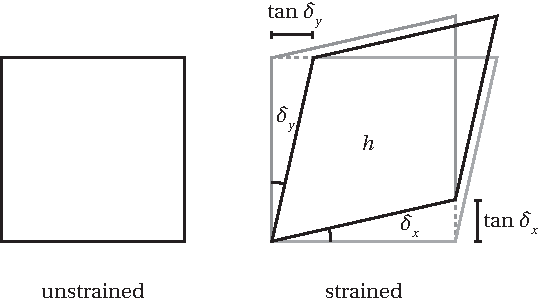
\includegraphics[]{seismology/figures/shear_strain.pdf}
    \caption{Shear strain.  As shear strain occurs in the $xy$-plane, points are rotated by and angle $\delta_x$ in the $y$ direction due to shear along the $y$-axis and rotated by an angle $\delta_y$ in the $x$ direction due to shear along the $x$-axis.  The total shear rotation is $\delta_x + \delta_y$.}
    \label{fig:shear}
\end{figure}

Now we can write the full strain tensor with all 9 components
\begin{align*}
    \vb{\epsilon} & =
    \begin{bmatrix}
        \epsilon_{xx} & \epsilon_{xy} & \epsilon_{xz} \\
        \epsilon_{yx} & \epsilon_{yy} & \epsilon_{yz} \\
        \epsilon_{zx} & \epsilon_{zy} & \epsilon_{zz}
    \end{bmatrix} \\
    & =
    \begin{bmatrix}
        \pdv{u_x}{x} &
        \frac{1}{2}\left( \pdv{u_y}{x} + \pdv{u_x}{y} \right) &
        \frac{1}{2}\left( \pdv{u_z}{x} + \pdv{u_x}{z} \right) \\
        \frac{1}{2}\left( \pdv{u_y}{x} + \pdv{u_x}{y} \right) &
        \pdv{u_y}{y} &
        \frac{1}{2}\left( \pdv{u_z}{y} + \pdv{u_y}{z} \right) \\
        \frac{1}{2}\left( \pdv{u_x}{z} + \pdv{u_z}{x} \right) &
        \frac{1}{2}\left( \pdv{u_y}{z} + \pdv{u_z}{y} \right) &
        \pdv{u_z}{z}
    \end{bmatrix}
\end{align*}

Just one additional note regarding shear.  Shear also causes a rotation of the body orthogonal to the sheared plane.  This angle is given by
\begin{align}
    \theta_{z} & = \delta_x - \delta_y \\
    & = \pdv{u_y}{x} - \pdv{u_x}{y} \\
    \theta_{y} & = \pdv{u_x}{z} - \pdv{u_z}{x} \\
    \theta_{x} & = \pdv{u_z}{y} - \pdv{u_y}{z}.
\end{align}
Note the similarity of the above equation to the curl.  We will return to this soon. 


\section{Elastic constants}

As strain occurs in one direction, a strain occurs in the two axes orthogonal to the original strained axis.  Think of this process like pulling taffy.  When you stretch the taffy in one direction, there is also a change in dimension in the other two axes.  The relationship between the strain in the original axis and the other two is a result of the material properties of the medium (Figure~\ref{fig:poisson}),
\begin{align}
    \nu & = -\frac{\epsilon_{yy}}{\epsilon_{xx}} \\
    \nu & = -\frac{\epsilon_{zz}}{\epsilon_{xx}}.
    \label{eq:poisson}
\end{align}
We call this relationship Poisson's ratio, $\nu$, and as we shall see it also relates the pressure and shear wave velocities through a medium.
\begin{figure}[hbtp]
    \centering
    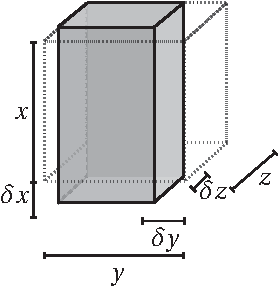
\includegraphics[]{seismology/figures/poisson.pdf}
    \caption{Dilation strain.  As strain occurs in the $x$-direction, $\epsilon_{xx} = \frac{\delta x}{x}$, a strain also occurs in the $y$- and $z$-directions, $\epsilon_{yy} = \frac{\delta y}{y}$ and $\epsilon_{zz} = \frac{\delta z}{z}$.  The strains are related by the Poisson ratio, $\epsilon_{xx} = -\nu \epsilon_{yy}$ and $\epsilon_{xx} = -\nu \epsilon_{zz}$.}
    \label{fig:poisson}
\end{figure}

As mentioned earlier, through Hooke's law, the stress and strain can be linearly related,
\begin{align}
    \sigma_{xx} & = E \epsilon_{xx} \\
    \sigma_{yy} & = E \epsilon_{yy} \\
    \sigma_{zz} & = E \epsilon_{zz}
    \label{eq:young}
\end{align}
where $E$ is a material constant called {\it Young's modulus} which is a measure of the tensile strength of a material (similar to a spring constant).  Combining Equations~\ref{eq:poisson} and \ref{eq:young}, we find that the strain in one dimension is related to stresses in all three by
\begin{align*}
    E \epsilon_{xx} & = \sigma_{xx} - \nu \sigma_{yy} - \nu \sigma_{zz} \\
    E \epsilon_{yy} & = \sigma_{yy} - \nu \sigma_{zz} - \nu \sigma_{xx} \\
    E \epsilon_{zz} & = \sigma_{zz} - \nu \sigma_{xx} - \nu \sigma_{yy}.
\end{align*}
Summing these three equations and dividing by three we have
\begin{equation*}
    E (\epsilon_{xx} + \epsilon_{yy} + \epsilon_{zz}) = 
    (1 - 2 \nu)(\sigma_{xx} + \sigma_{yy} + \sigma_{zz}) .
\end{equation*}

If the pressure is hydrostatic then $\sigma_{xx} = \sigma_{yy} = \sigma_{zz} = -P$.  Recall from Equation~\ref{eq:dilation}, $\phi = \epsilon_{xx} + \epsilon_{yy} + \epsilon_{zz}$.  Inputting these two relations into the above result, we see
\begin{equation*}
    E \phi = -3 p (1 - 2 \nu) .
\end{equation*}

We will introduce a material constant called the bulk modulus, $K$, that relates the hydrostatic pressure to the dilation,
\begin{equation}
    p = -K \phi,
\end{equation}
which we input into the previous result,
\begin{equation}
    E = 3 K (1 - 2 \nu) .
\end{equation}
The bulk modulus may also be defined in terms the Lam{\'e} constants,
$\lambda$ and $\mu$ by
\begin{equation}
    K = \lambda + \frac{2}{3} \mu ,
\end{equation}
where $\mu$ is also known as the shear modulus.

Just as we defined a proportionality constant for the dilation, we can define a {\it shear modulus} such that
\begin{align}
    \sigma_{xx} & = \mu \epsilon_{xx} \\
    \sigma_{yy} & = \mu \epsilon_{yy} \\
    \sigma_{zz} & = \mu \epsilon_{zz} .
    \label{eq:shear}
\end{align}
It can be shown that the shear modulus is related to Young's modulus and the
Poisson's ratio by
\begin{equation}
    E = 2 \mu (1 + \nu) .
\end{equation}


\section{Wave Equation}

We can write the displacement field as a combination of a scalar potential, $\phi$, related to the dilation and a vector potential, $\vb{\psi}$, related to the shear,
\begin{equation}
    \vb{u} = \grad \phi + \curl \vb{\psi} .
\end{equation}
The wave equation is defined as
\begin{equation}
    \pdv[2]{u}{t} = V^2 \nabla^2 \vb{u},
\end{equation}
where $V$ is the velocity of the wave
\begin{equation}
    V = \sqrt{\frac{E}{\rho}}.
\end{equation}

Treating each separately, we can write the wave equations for $P$-waves as
\begin{equation}
    \pdv[2]{\phi}{t} = V_P^2 \nabla^2 \phi,
\end{equation}
and for $S$-waves,
\begin{equation}
    \pdv[2]{\vb{\psi}}{t} = V_S^2 \nabla^2 \vb{\psi},
\end{equation}
where $V_P$ and $V_S$ are the $P$- and $S$-wave velocities, respectively.
The wave velocities are related to the material properties by
\begin{align}
    V_P & = \sqrt{\frac{K + \frac{4}{3} \mu}{\rho}} \\
    V_S & = \sqrt{\frac{\mu}{\rho}}.
\end{align}

We come to a peculiar solution that the wave velocities are related to the inverse of the density.  This may seem counter-intuitive and it is; however, the bulk modulus is related to the density by
\begin{equation}
    K = -V \dv{P}{V} = \rho \pdv{P}{\rho}.
\end{equation}

All of the material constants and the wave equations above have been introduced assuming a isotropic medium.  If the medium is anisotropic, then the material constants have different values in different directions.  Anisotropy is generally occurs in minerals because crystal structures are not uniform but have different shape systems.  While some minerals are isotropic (e.g.\ garnet, halite), most are not.  Major rock forming minerals such as quartz, olivine, and particularly micas have substantially different physical properties that correspond to their crystallographic axes.  As such, seismic waves may propagate at different velocities in different directions.  However, many rocks are a random aggregate of crystal orientations of various minerals which allows for isotropic approximations despite individual anisotropic components.

\section{Earthquake Seismology}
The subject of earthquake seismology is incredibly vast and one of the most useful methods by which we can study the structure and processes occurring within the Earth.  There is no way we can even cover a representative fraction of the subject in a few lectures.  Therefore, I have decided to focus on only a few aspects in some detail.  

\subsection{Seismic Cycle}
Earthquakes triggering is a complex mechanism. However, it is the same mechanisms that generate millimeter or multi-kilometer ruptures. 

During the \emph{interseismic stage}, which makes up most of the cycle, a loading (e.g. a force accumulation) occurs on asperities locating on the shallow part of the fault. This part is "locked", although some deformations affect the deeper part of the fault via a aseismic creep (figure \ref{figure_seismic_cycle}b). 

After a long period of time, the rock failure threshold $\sigma_c$ on an asperity is reached, the rock break and a slip begin at this point. This phase, the \emph{coseismic stage}, lasts few second to minutes and meters of slip on the fault "catch up" with the few mm/yr of motion that occurred during the interseismic stage (figure \ref{figure_seismic_cycle}c). This quick emission of energy generates seismic waves and unloads the asperities on a quantity called "stress drop" ($\Delta \sigma$).  When the energy released become too low to propagate the rupture, the slip stops and the asperity begin again to accumulate stresses.

Finally, a \emph{postseismic stage} occurs after the earthquake, and aftershock and transient afterslip occur for a period of years before the fault settles into its steady interseismic behavior again.
\begin{figure}[h]
    \centering
    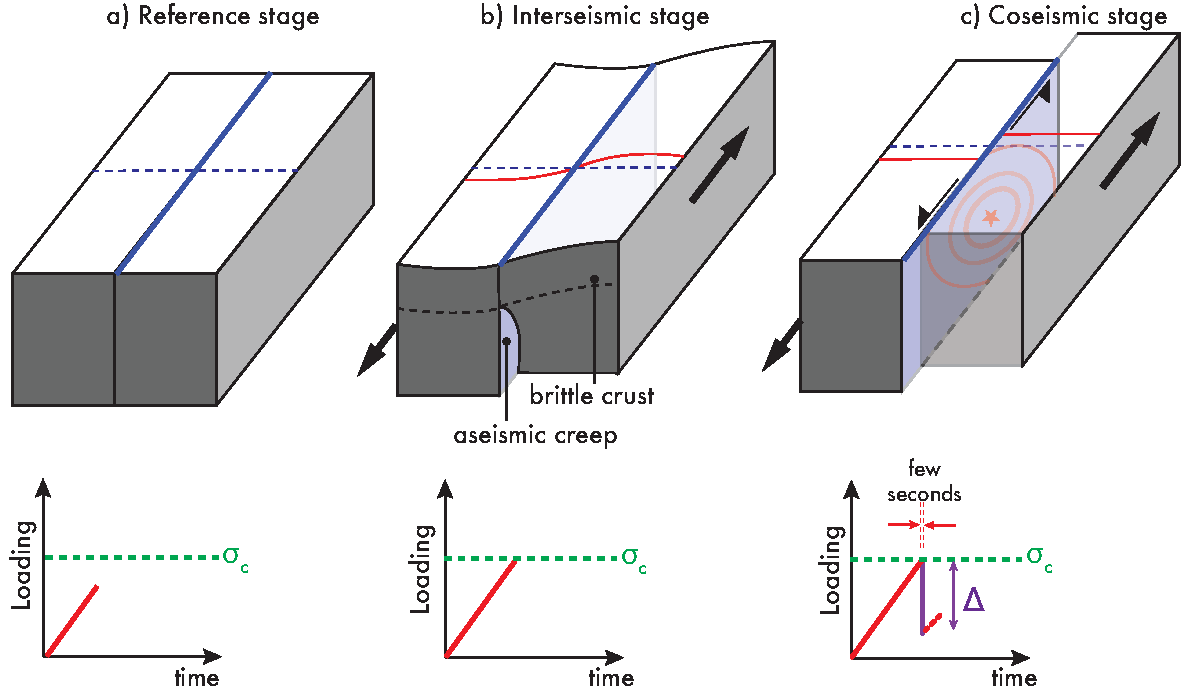
\includegraphics[trim = 5mm 180mm 0mm 0mm, clip,scale=0.6]{seismology/figures/seismic_cycle.pdf}
    \caption{From a initial stage (a), a fault accumulates loading on the locked part during the interseismic stage (b), and a slowly deformation appears on the surface. When the rock failure on the fault is reached, the coseismic stage (c) begin and the fault breaks---it's an earthquake birth.}
    \label{figure_seismic_cycle}
\end{figure}

These types of deformations can be observed by geodesy. For example, GPS stations can recorded deformation for some years for specific points on the surface, and radar interferometry (measuring precisely the displacement between two pictures of the same areas) can showed the co-seismic effect after an earthquake (Figure~\ref{figure_seismic_cycle_subduction}). 

\begin{figure}[h]
    \centering
    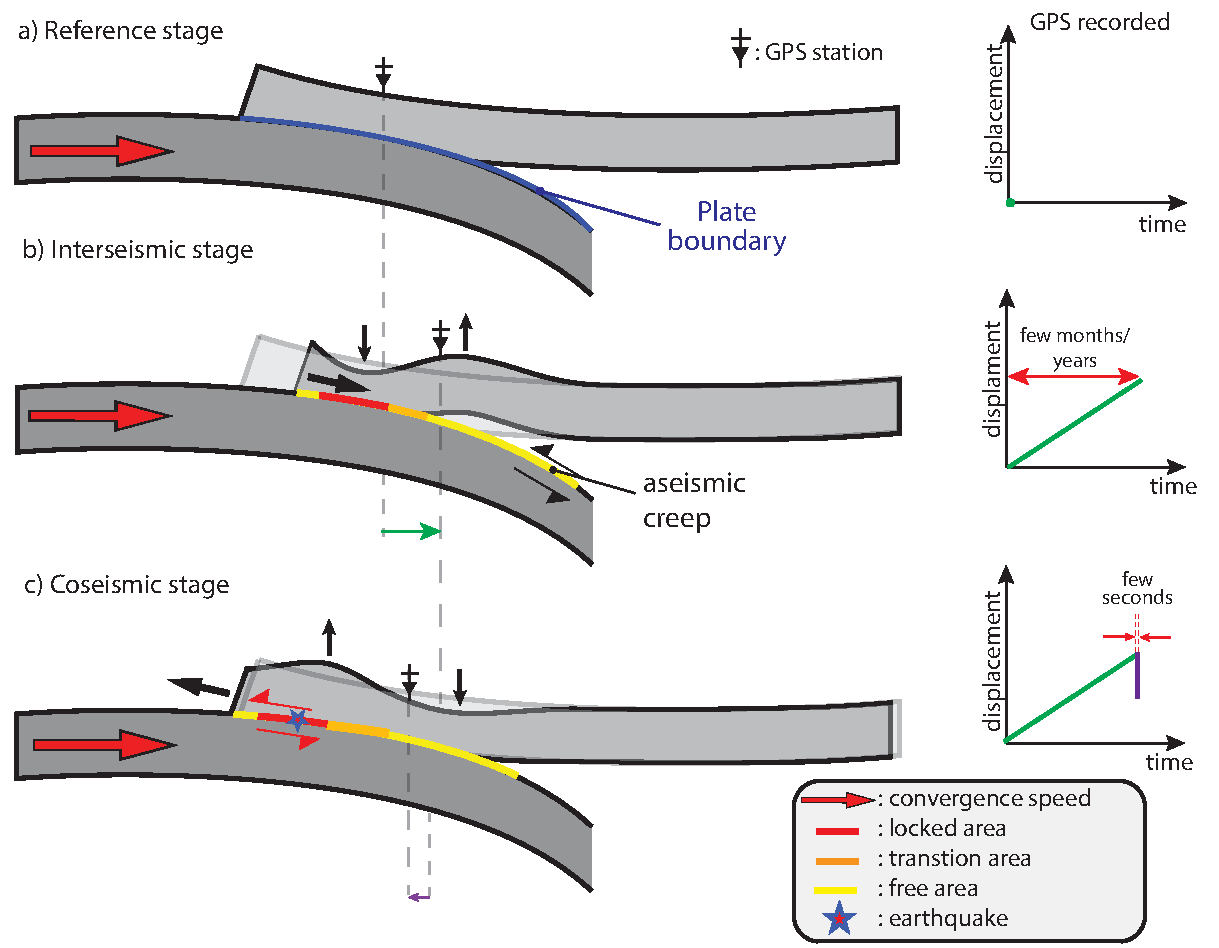
\includegraphics[trim = 5mm 120mm 0mm 0mm, clip,scale=0.5]{seismology/figures/seismic_cycle_subduction.pdf}
    \caption{Seismic cycle representation in the subduction context.  Displacements can be observed by geodetic method as GPS station. }
    \label{figure_seismic_cycle_subduction}
\end{figure}

\subsection{Magnitude}
More the energy released by earthquake is important, more earthquake will be strong. Indeed, this energy is used to break the rock and spread the rupture. A common equation to quantify this energy is the \textit{seismic moment} $M_0$:
\begin{equation}
    M_0= \mu \times  \bar{d} \times S
\end{equation}
where $\mu$ is the shear modulus (or modulus of rigidity), $\bar{d}$ is the average fault displacement on the fault with area $S$. The unit of the seismic moment is N.m (but older references express $M_0$ in \si{dyne.cm}).

For historical reasons, the most well-known measure of earthquake size is the earthquake magnitude. There are now several different types of magnitude scales but all are related to the largest amplitude that is recorded on a seismogram.  This is one of the easiest things to measure and is one reason for the continued popularity of magnitude scales.

The earliest magnitude scale and introduced by Charles Richter in 1935, is the \textit{local magnitude} $M_L$, based on the maximum amplitude $A$ (often S-waves) in micrometers recorded on standard short period (1 sec) seismometer and corrected with a standard value $A_0$ depending of the distance between source and the receiver as :
\begin{equation}
    M_L= \log_{10} (A/A_0)
\end{equation}
This magnitude is correct for earthquakes less than 1000 kilometers from the instrument measuring the earthquake.

But with time, other magnitudes types appeared. The first one is the
\textit{body-wave magnitude} $m_b$, based on the measure of the amplitude of the
P body waves generated by the earthquake, using :
\begin{equation}
    m_b= \log_{10}(A/T) + Q(D,h)
\end{equation}
where T (in second) is the period of the wave being measured, $A$ is its amplitude and $Q(D,h)$ is a correction factor that is a function of distance, $D$ (in degrees), between epicenter and station and focal depth, $h$ (in kilometers), of the earthquake

The \textit{surface wave magnitude} $M_S$ is measured using the largest
amplitude of the surface waves and its general formula is : 
\begin{equation}
    M_S= \log_{10} (A/T) + 1.66 \log_{10} (D) +3.3
\end{equation}

When initially developed, these magnitude scales were considered to be equivalent; in other words, earthquakes of all sizes were thought to radiate fixed proportions of energy at different periods. But it turns out that larger earthquakes, which have larger rupture surfaces, systematically radiate more long-period energy. Thus, for very large earthquakes, body-wave magnitudes badly underestimate true earthquake size; the maximum body-wave magnitudes are about 6.5--6.8. In fact, the surface-wave magnitudes underestimate the size of very large earthquakes; the maximum observed values are about 8.3--8.7.

To avoid these saturation problems, Kanamori in 1977 proposed the \textit{moment
magnitude} $M_w$ using the seismic moment $M_0$:
\begin{equation}
    M_w= \frac{2}{3} \log_{10} (M_0) - 6.1
\end{equation}
Now, this final formula is the most commonly magnitude used and it allows to estimate that the energy increase of factor $\times 32$  between a magnitude $M_w$ and $M_w+1$  (see table \ref{table_Seismic_Energy}).

\begin{table}[hbpt]
    \centering
    \caption{Examples of values for different historical eathquakes. (from Stein
    and Wysession 2003)}
    \label{table_Seismic_Energy}
    \begin{tabular}{ccccc}
        \toprule 
        \textbf{Earthquake} &
        \textbf{Fault Area} (km$^2$) &
        \textbf{Average} &
        \textbf{Seismic moment} &
        \textbf{Moment} \\ 
        & (length $\times$ width) & dislocation (m) & (\si{dyne.cm}), $M_0$ & magnitude,
        $M_w$ \\ 
        \midrule 
        Truckee, 1966 & 10 $\times$ 10 & 0.3  & $8.3 \times 10^{24}$ & 5.9 \\ 
        San Fernando, 1971 & 20 $\times$ 14 & 1.4  & $1.2 \times 10^{26}$ & 6.7 \\ 
        Loma Prieta, 1989 & 40 $\times$ 15 & 1.7 & $3.0 \times 10^{26}$ & 6.9 \\ 
        San Francisco, 1906 & 450 $\times$ 10& 4 & $5.4 \times 10^{27}$  & 7.8 \\ 
        Alaska, 1964 & 500 $\times$ 300 & 7 & $5.2 \times 10^{29}$ & 9.1 \\ 
        Chile, 1960 & 800 $\times$ 200 & 21 & $2.4 \times 10^{30}$ & 9.5 \\ 
        \bottomrule 
    \end{tabular} 
\end{table}

\subsection{Earthquake statistics}
\subsubsection{Relation between magnitude and frequency}
If you look at the number of earthquake per magnitude for a specific region and for a period of time,  you can observe that the number of events of low magnitudes is more important than for high magnitude. This observation was quantified by Gutenberg and Richter in the 1940s via the following relation known as the \textit{Gutenberg and Richter law} : \begin{equation} \log_{10} N=  a - b \times M \end{equation} where $N$ is the number of earthquakes with magnitude greater than $M$ occurring in a given time, $a$ depends on the number of earthquakes in the time and region sampled and the slope $b$ is generally about 1 (figure \ref{figure_GR_law}).

\begin{figure}[hbpt]
    \centering
    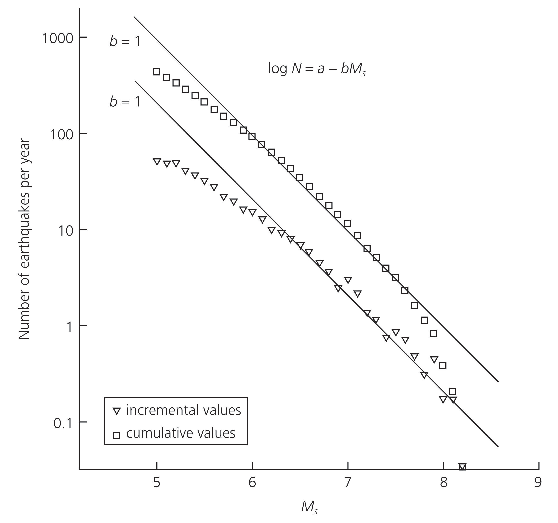
\includegraphics[trim = 0mm 0mm 0mm 4mm, clip,scale=0.9]{seismology/figures/4_7_01.pdf}
    \caption{Frequency-magnitude plot for all earthquakes with $M_S \geqslant 5.0$ during 1968-97 listed in the catalog of the National Earthquake Information Center (from Stein and Wysession 2003).}
    \label{figure_GR_law}
\end{figure}

\subsubsection{Aftershocks distribution}
After an earthquake occurrence (called mainshock), following events triggered by this earthquake, (called aftershocks) have a characteristic distribution in size and time. The largest aftershocks are usually more than a magnitude unit smaller than the mainshock, and the size distribution is agreed with the Gutenberg-Richter law, although the energy released by the aftershock is usually less than 10 $\%$ of that the mainshock.

Most of the aftershocks occur after the mainshock, and the number of events $n(t)$ is described by the relation : \begin{equation} n(t)=  \frac{K}{(t+c)^p} \end{equation} where $p$ is typically about 1, $K$ is the productivity parameter and $c$ is a constant. This law is called the Omori-Utsu law and can be observed after any earthquake (figure \ref{figure_aftershock_distribution}).
\begin{figure}[hbpt]
    \centering
    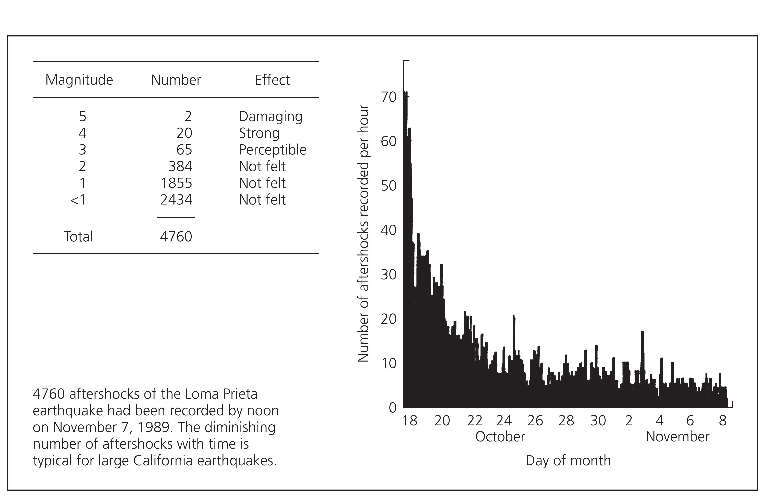
\includegraphics[trim = 2mm 2mm 2mm 8mm, clip,scale=1]{seismology/figures/4_7_08.pdf}
    \caption{Graphic showing the number and distribution aftershock in 22 days after the 1989 Loma Prieta earthquake as functions of magnitude and time (from Stein and Wysession 2003).}
    \label{figure_aftershock_distribution}
\end{figure}

It is important to know that the Earth is perpetually close to the rupture and small stress variations can trigger earthquakes.  A mainshock occurrence perturbs the stress for a specific region, and more the mainshock is important, more the perturbed region will be spread. A first perturbation mechanism is due to the dynamic stress variations produced by the seismic waves of the mainshock.  This phenomenon allows to explain aftershock occurrences in far field.  The other mechanism is called the static stress variations and corresponds to the variations due to the coseismic displacement. The coseismic displacements change the shear and normal stresses for faults present in the perturbed region by mainshock.  These variations of shear stress ($\Delta \tau_s$) and normal stress ($\Delta \sigma_n$) allows to estimate a parameter called the Coulomb stress changes ($\Delta  CFF$) with the equation:
\begin{equation}
    \Delta CFF = \Delta \tau_s + \mu' \Delta \sigma_n
\end{equation}
where $\mu'$ is the effective coefficient of friction. This value of $\Delta  CFF$ can be positive or negative and not really high (usually less than 1 bar only) but consistent observations between the region where the $\Delta  CFF$ is positive and the aftershocks locations were observed is some cases (as in 1992 Landers earthquake, in California, see figure \ref{figure_Coulomb_map}).
\begin{figure}[hbpt]
    \centering
    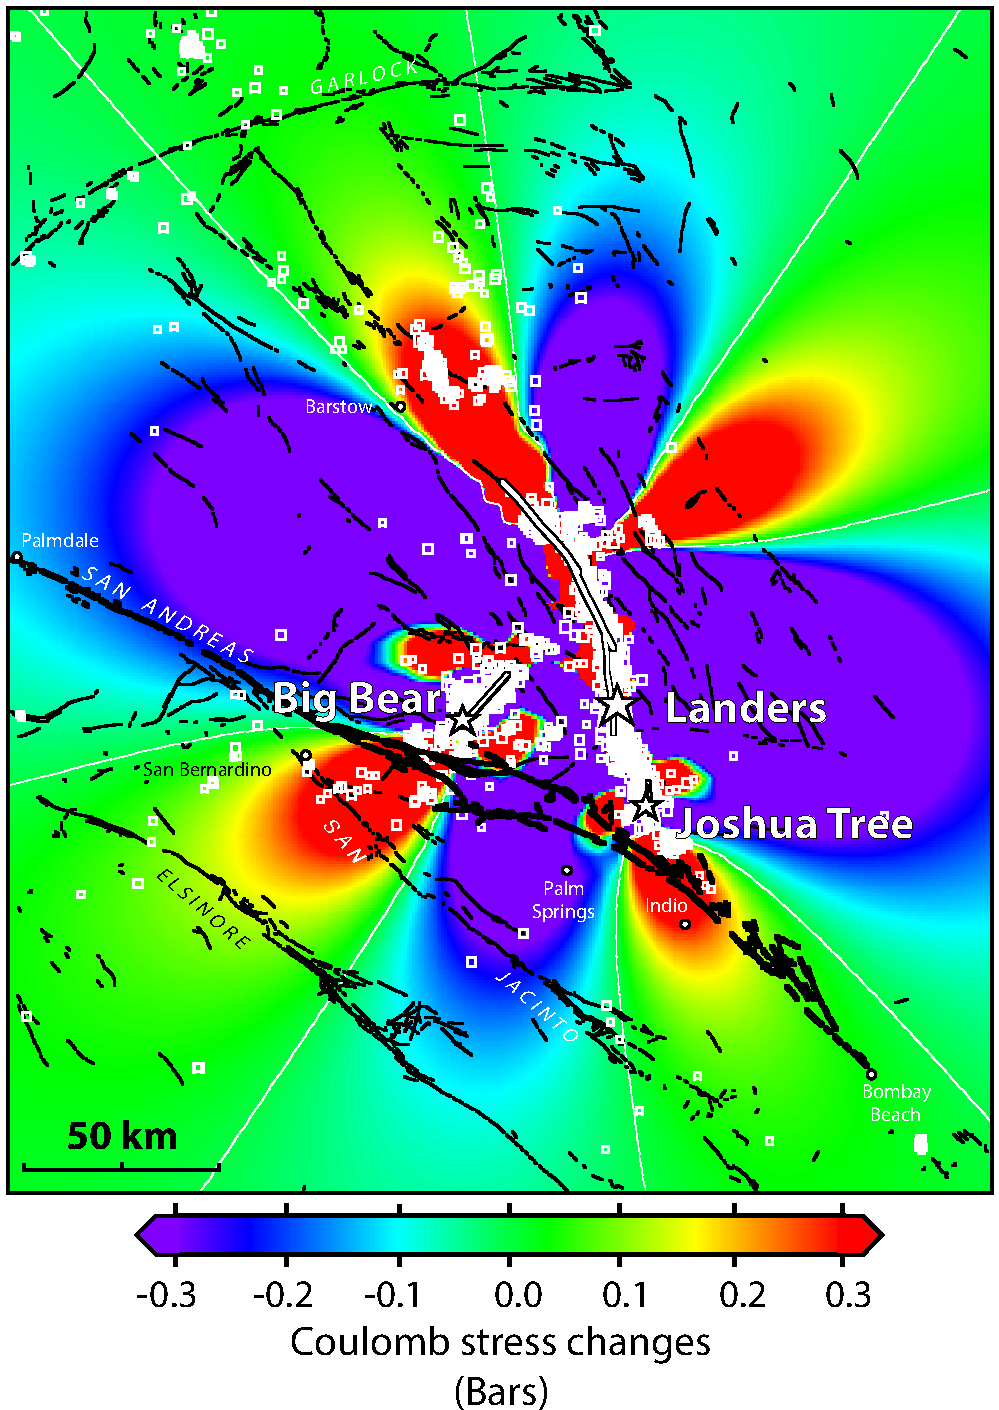
\includegraphics[trim = 25mm 10mm 23mm 20mm, clip,scale=0.5]{seismology/figures/Coulomb_Landers.pdf}
    \caption{Map of Coulomb stress changes after the occurrence of Joshua Tree,
    Landers and Big Bear earthquake. White squares indicate locations of
    aftershocks (from King et al, 1994).}
    \label{figure_Coulomb_map}
\end{figure}


\subsection{Seismograms}
The release of energy during an earthquake creates both $P$- and $S$-waves.  As
these waves travel through the earth, they reflect and refract as they interact
with changes in seismic velocities and/or acoustic impedance altering their
path, and possibly the type of wave itself.  As these waves travel through the
various layers within the Earth, they speed up and slow down in response to
these changes in velocity.  In addition to the changes in velocity the distance
the wave travels alters the time it takes for a mantle phase to reach a
seismometer.  Because rays traveling in different paths can arrive at very
similar times, we give the individual rays names based on the specific layers of
the Earth with which they interact.  An example of several phases are shown in
Figure~\ref{fig:phases}.  The naming scheme for ray paths are given in
Table~\ref{tab:phases}.
\subsection{Phases}
\begin{figure}[hbt]
    \centering
    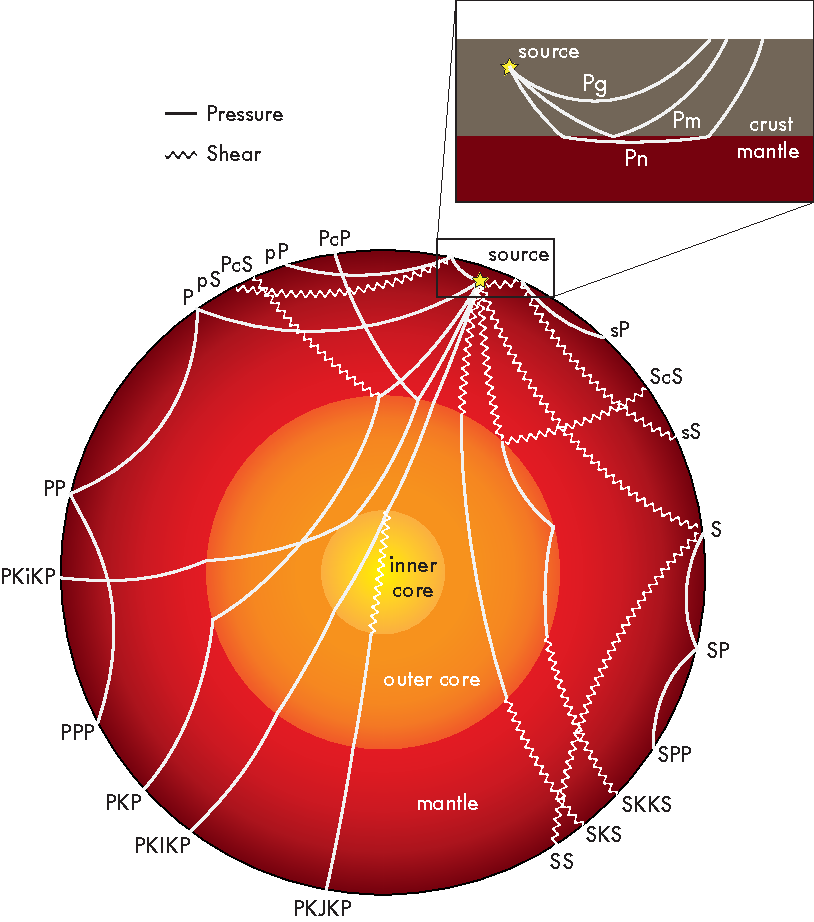
\includegraphics[]{seismology/figures/phases.pdf}
    \caption{Naming of seismic phases.  Inset shows naming scheme for selected
    crustal phases: $Pg$, internal crustal refraction; $Pm$, reflection off
    Moho; and $Pn$, critical refraction at Moho.}
    \label{fig:phases}
\end{figure}
\begin{table}[hbt]
    \centering
    \caption{Convention for seismic phases.}
    \label{tab:phases}
    \begin{tabular}{ll}
        \toprule
        \textbf{Key} & \textbf{Path} \\ 
        \midrule
        p   & short upgoing $P$-wave reflection at surface \\
        P   & $P$-wave in the mantle \\
        K   & $P$-wave in the outer core \\
        I   & $P$-wave in the inner core \\
        s   & short upgoing $S$-wave reflection at surface \\
        S   & $S$-wave in the mantle \\
        J   & $S$-wave in the inner core \\
        c   & reflection off mantle-outer core boundary \\
        i   & reflection off outer-inner core boundary \\
        \bottomrule
    \end{tabular}
\end{table}
\begin{figure}[hbt]
    \centering
    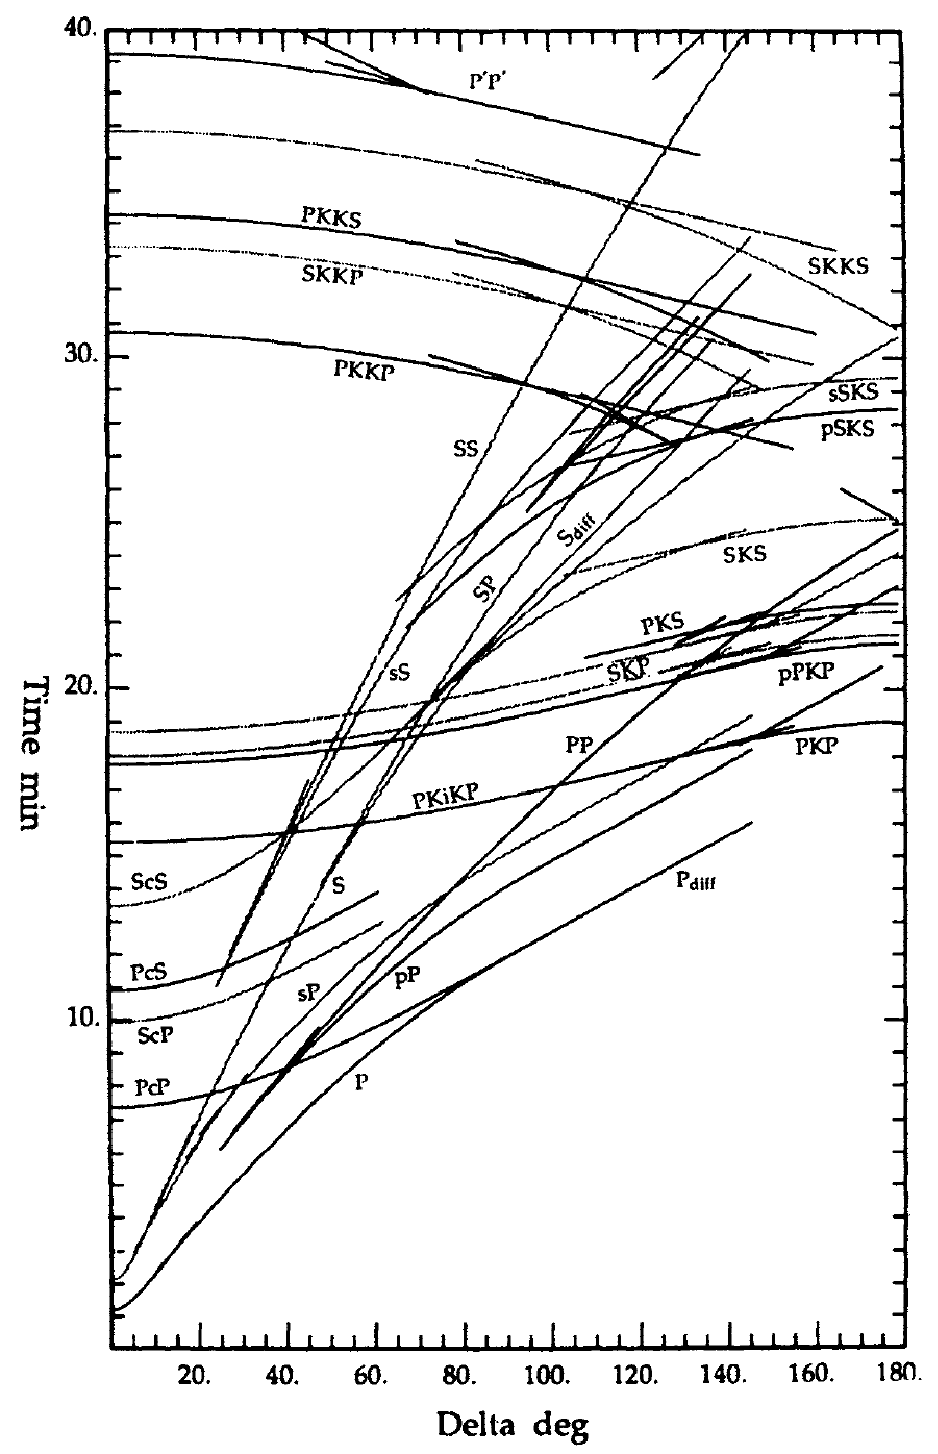
\includegraphics[]{seismology/figures/phase_travel_times.pdf}
    \caption{Estimated travel times for various phases as a function of
    epicentral difference. From \citet{Kennett&Engdahl1991}.}
    \label{fig:phasett}
\end{figure}

The combination of all these phases arriving at a single station are what build
a seismogram.  As you can imagine, the result can be quite complex
(Figure~\ref{fig:seismogram}).
\begin{figure}[hbt]
    \centering
    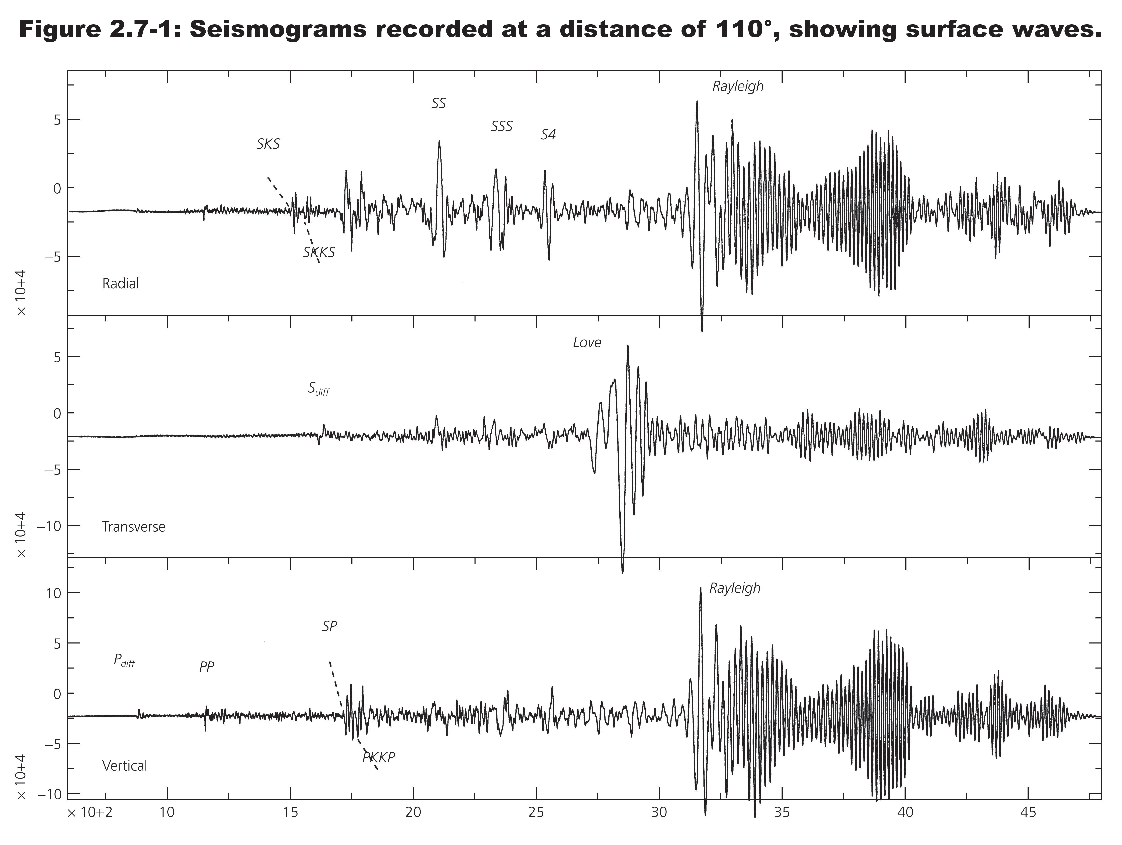
\includegraphics[width=\textwidth]{seismology/figures/seismograms.pdf}
    \caption{A seismogram with several key phases identified. From
    \citet{Stein&Wysession2003}.}
    \label{fig:seismogram}
\end{figure}


\subsection{Locating Earthquakes}
When an earthquake occurs, waves spread spherically (sort of) from the source.
The time that it takes a wave to reach an observation point (seismometer) is
proportional to the distance from the source,
\begin{equation}
    d = v t,
\end{equation}
where $d$ is the distance from the source, $t$ is the travel time of the wave
and $v$ is the velocity of the wave.  However, we typically do not know the time
of origin of the earthquake {\it a priori}.  Hence, we need some other way to
estimate distance.  Luckily, we have two types of waves with the same origin
time, which allows us to use the difference between time travels of the two
waves to estimate distance.  To do so we can write the travel time for each wave
from the source as
\begin{align}
    t_P &= \frac{d}{V_P} \\
    t_S &= \frac{d}{V_S}.
\end{align}
We can then use the above relationship to solve for the distance.
Using a relatively standard assumption for the ratio in velocities, it
can be shown that the distance from a station to the epicenter is
\begin{equation}
    d = \frac{t_S - t_P}{\sqrt{3} - 1} \bar{V}_P ,
\end{equation}
where $\bar{V}_P$ is the average $P$-wave velocity.  Note: this equation only
works for stations relatively near the source ($<$20$^\circ$) because as the
distance to the source increases the curvature of the Earth comes into play.
\FloatBarrier


\subsection{Focal Mechanisms}
A seismogram (seismic response) is a complicated observed response due to an
earthquake or from an exploration source.  Mathematically, a seismogram is
represented as
\begin{equation}
    \coreeq
    \mlbox[labelstyle={xshift=-2cm},
        linestyle={out=270,in=90, latex-}]{u(t)}{displacement (seismogram)} =
    \mlbox[labelstyle={xshift=-2cm, yshift=-1ex, below of=m\themathLableNode, below of=m\themathLableNode},
        linestyle={out=90,in=270, latex-}]
        {s(t)}{seismic source} \ast
    \mlbox[labelstyle={yshift=-2ex, below of=m\themathLableNode, below of=m\themathLableNode}]
        {G(t)}{Earth's properties} \ast
    \mlbox[
        labelstyle={xshift=2cm, yshift=-1ex, below of=m\themathLableNode, below of=m\themathLableNode},
        linestyle={out=90,in=270, latex-}]
        {Q(t)}{attenuation} \ast 
    \mlbox[]{r(t)}{seismometer/geophone response} ,
\end{equation}
where $G$ is a Green's function related to the Earth's structure including the
velocity and impedence distribution.  Note `$\ast$' here is not a multiplication
but a convolution. Obviously, this will be quite challenging to solve since we
can control $r$ and $s$ for exploration seismic studies but only $r$ for
earthquake seismology.  The attenuation $Q$ is the decrease in the amplitude of
the seismic wave as a result of viscous dissipation.

\ntextbox{Convolution}{
    A convolution describes the way in which a source wave is transformed as it
    passes through some medium, resulting in the response we measure.  The
    convolution of two time-series, $u$ and $v$, is defined by
    \[
        u(t) \ast v(t) = \int_{-\infty}^{\infty} u(\tau) v(t - \tau) \dd{\tau} .
    \]
    Since we typically use digital recordings, we can write a discrete convolution
    as
    \[
        u_i \ast v_i = \sum_{j=-\infty}^{\infty} u_{i-j} v_j ,
    \]
    where $u_i = u(t_i)$ and $v_i = v(t_i)$, respectively.  The sampling interval in
    time $\Delta t = t_{i+1} - t_i$ is constant.  The subscript $j$ represents a
    shift in integral values of $\Delta t$.  Although the definition goes from $\pm
    \infty$, we do not really perform the integration to infinity since our time
    series are finite and we assume zero magnitude on either end.  An example is
    given below in~\ref{fig:conv}.
    \vspace{4ex}

    \begin{center}
        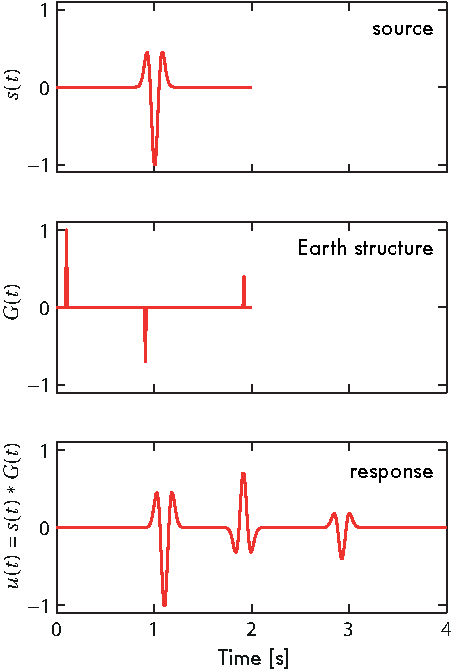
\includegraphics[]{seismology/figures/convolution.pdf}

        \textbf{Figure~\thefigure:} Convolution of two functions to produce a third.
        \label{fig:conv}
    \end{center}

    Convolutions have the following properties, $u \ast v = v \ast u$ and $u \ast (v
    \ast w) = (u \ast v) \ast w$.

    Convolutions are often made simpler by applying a Fourier transform from the
    time to frequency domain.  This has the advantage of turning our integral into a
    simple multiplication,
    \[
        u(\omega) = r(\omega) a(\omega) G(\omega) s(\omega) .
    \]
}{core}

Consider the seismic source and Earth's structure in Figure~\ref{fig:conv}. For
the moment, we will ignore the response of our seismic recorder and the
attenuation. The convolution of the source with the Earth's structure result in
a seismogram.  The sign of the Earth's structure and source affect the sign of
the convolved signal in the seismogram.  This example is quite simple resulting
in a separation of time between the arrival of each wave.  However, in reality,
the response can be significantly more complicated as the convolved response
from each interface in the Earth begins to overlap slightly for shorter period
waves or dramatically for longer period waves as shown in
Figure~\ref{fig:convw}.
\begin{figure}[htbp]
    \centering
    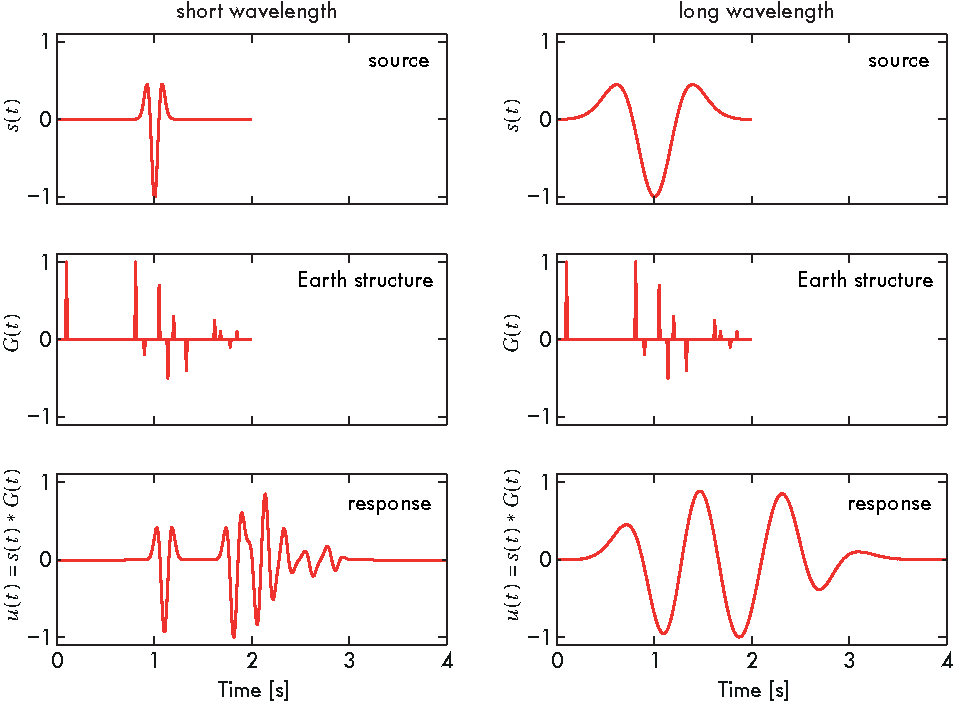
\includegraphics[]{seismology/figures/convolution_wavelength.pdf}
    \caption{Convolution of a seismic source (top row) with a Earth's structure
    (middle row) to produce a synthetic seismogram.  Note this seismogram
    ignores the effect of attenuation and reciever response for simplicity.
    Left column is a high frequency, short period wave; right column is a low
    frequency, long period wave.}
    \label{fig:convw}
\end{figure}

For an earthquake, $s(t) = M(t)$ is the moment tensor.  In earthquake
seismology, we know neither $G$ nor $M$ but wish to know both.  Focal mechanisms
are a way to graphically illustrate particular properties of $M$.

When rupture occurs along a fault, the first motion of pressure wave
(compression or rarefaction) depends upon its location relative to the fault
plane and the source location.  Imagine a point rupture on a fault plane.  In
the direction of motion of the fault slip, the first motion is a compression.
In the direction opposite of the fault slip, the first motion is a rarefaction.
Hence seismograph stations that lie within certain orientations of relative to
the earthquake's source and fault plane experience different first motions (or
polarity).
\FloatBarrier
\begin{figure}[hbtp]
    \centering
    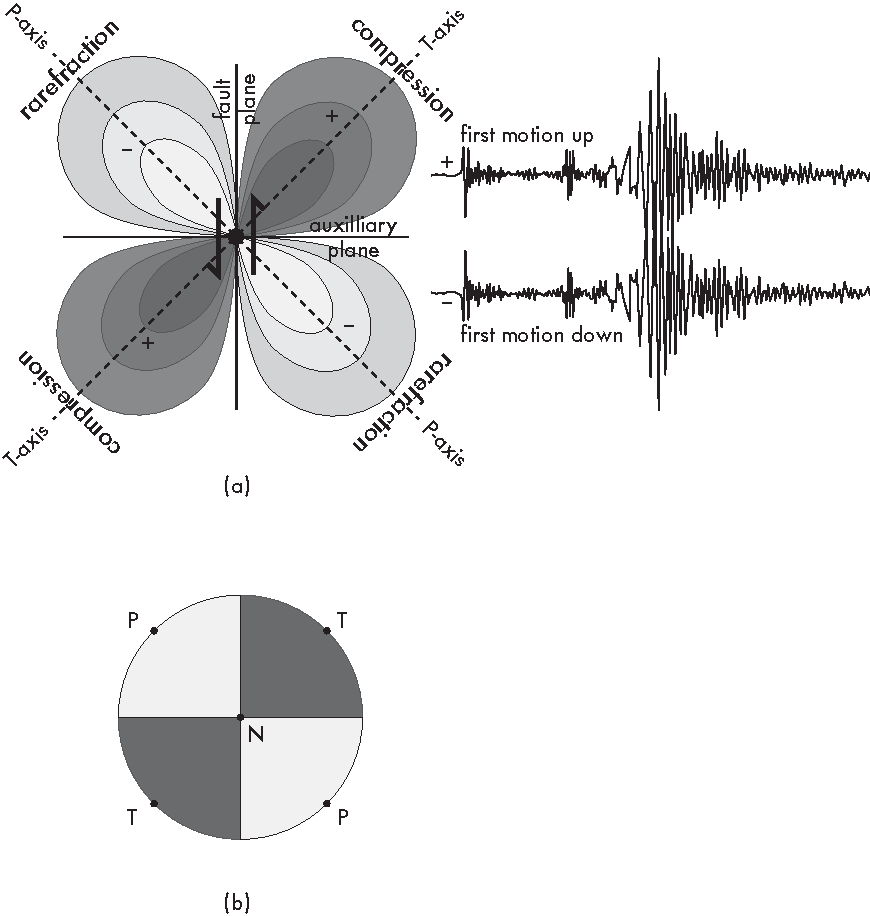
\includegraphics[]{seismology/figures/polarity.pdf}
    \caption{The $P$-wave radiation pattern from double couple mechanism (typical
    of most earthquakes) and its relation to the focal mechanism solution.
    Compression and rarefaction refer to the first motion of the elastic wave.
    The P- and T-axes are the maximum compressional and tensional axes,
    respectively, and refer to the press stress state.}
    \label{fig:polarity}
\end{figure}

Using the collective polarity observations from a global seismic network, we can
estimate the type of rupture and the orientation of the fault plane.  Graphically
we represent this with a focal mechanism (lovingly referred to as beach balls).
Mathematically, the focal mechanisms are related to the moment tensor solution
which relates to the type and orientation of the fault.  As a result the focal
mechanisms can look quite different from each other (Figure~\ref{fig:fm}). 
\begin{figure}[hbtp]
    \centering
    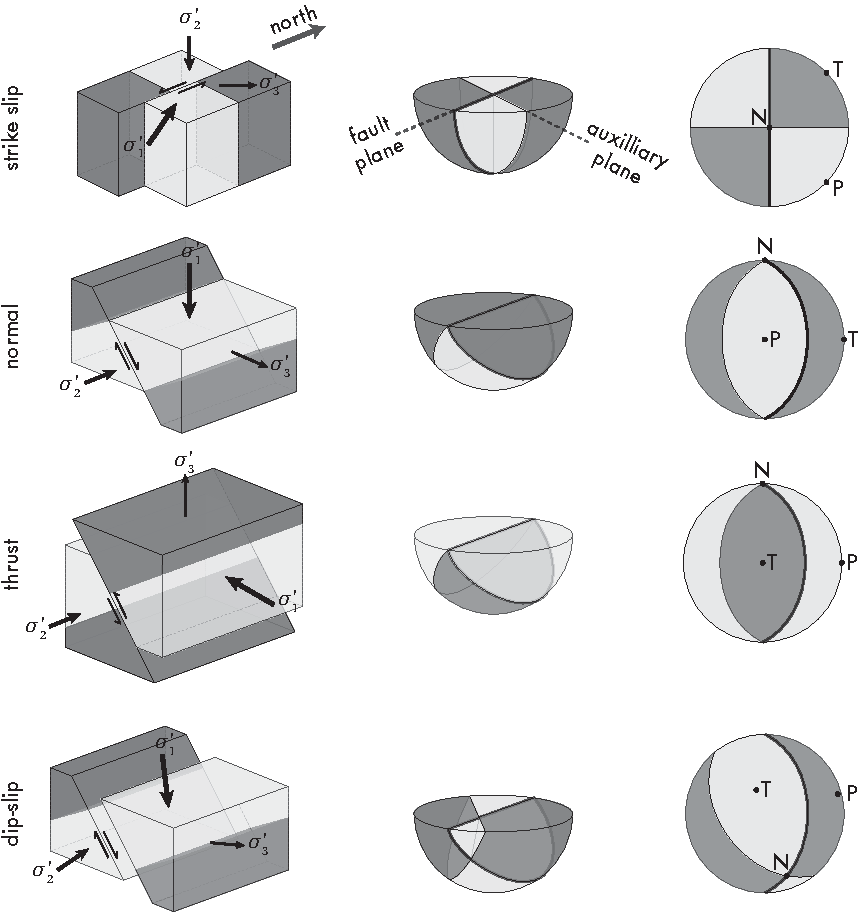
\includegraphics[]{seismology/figures/beach_balls1.pdf}
    \caption{Focal mechanisms solutions for different types of faulting and their
    relationship to maximum ($\sigma_1$) and minimum ($\sigma_3$) stresses.}
    \label{fig:fm}
\end{figure}

The center of each quadrant of the focal mechanism represents the locations of
the P- (compressional) and T- (tensional) axes of the pre-stressed state which
generated the earthquake.  Because the P- and T-axes relate to the pre-stressed
state rather than the stress during the earthquake rather than the quadrants of
first motions indicated by the color of the quadrant.  The intersection of all
four quadrants represents the neutral axis and is sometimes labeled N (not to be
confused with north).  The focal mechanisms can be used to estimate the strike
and dip of the fault as well.  Since there are four quadrants, there is a
90$^\circ$ ambiguity of the fault plane, one of which is the true fault plane
and the other we call the auxiliary plane.

Consider the case where we can decompose (rotate) our stress tensor into the
principle stresses
\begin{equation*}
    \vb{\sigma} =
    \begin{bmatrix}
        \sigma_1 & 0 & 0 \\
        0 & \sigma_2 & 0 \\
        0 & 0 & \sigma_3
    \end{bmatrix},
\end{equation*}
such that $\sigma_1 > \sigma_2 > \sigma_3$.  If we subtract the mean of the three stresses then we have the deviatoric stress that we typically care about in geoscience
\begin{equation}
    \text{maximum tension }
    \sigma_1' > \sigma_2' > \sigma_3'
    \text{maximum compression }.
\end{equation}
In the ideal case, the $\sigma_1'$ and $\sigma_3'$ stress directions would directly relate to the P- and T-axes; however, in rocks the failure planes are not oriented 45$^\circ$ to the rupture, but at an angle typically between 20$^\circ$ and 30$^\circ$.

There are a number of other sources types some of which are shown in Figure~\ref{fig:fm2}.  Not all of these source types have three stress axes as many of these solutions result from cylindrical or spherically symmetric stress patterns.
\begin{itemize}
    \item Technically the majority of an earthquake source is a double couple mechanism which has four quadrants (quadrupole).  However, because fault surfaces are not purely planar and compressible fluids often exist along fault zones the source mechanisms can be a bit more complicated.  Since we assume very little volume change, most earthquakes can by modeled by some component of a CLVD (compensated linear vector dipole) solution in addition to the double couple.

    \item Purely expansive mechanisms to identify nuclear blasts by ``rogue'' nations.  The purely contractional (implosion) mechanism may more closely represent a mine collapse (although they often appear more like crack closures).

    \item Crack opening mechanisms may be important in induced seismicity due to fracking or other fluid injection sites.  Additionally, magma injection may also appear as a crack opening mechanism.  Crack closing mechanisms may result from extraction of fluids.
\end{itemize}
\begin{figure}[hbtp]
    \centering
    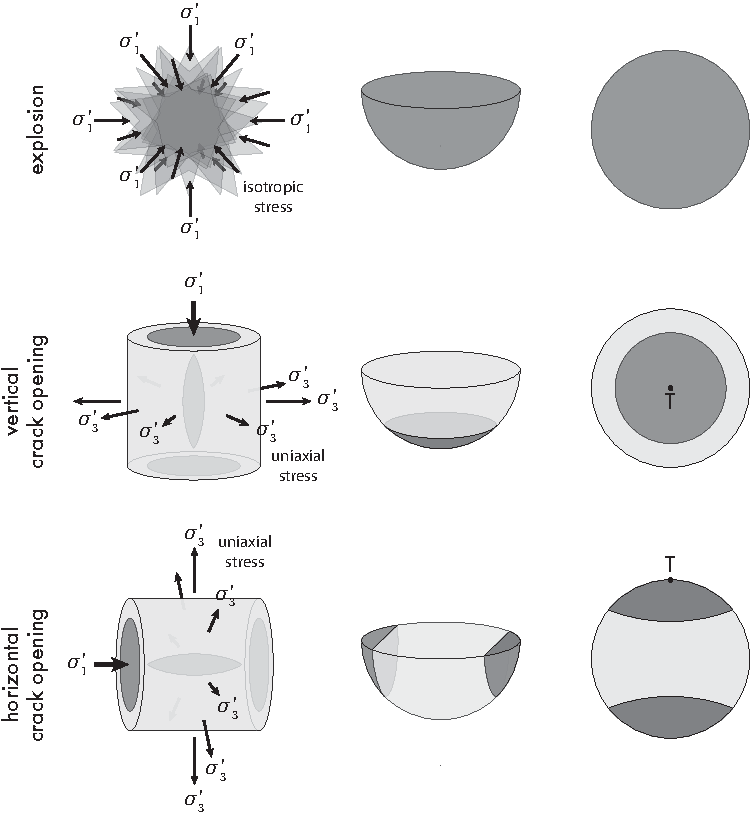
\includegraphics[]{seismology/figures/beach_balls2.pdf}
    \caption{Focal mechanisms solutions for sources other than pure end-member
    fault types.}
    \label{fig:fm2}
\end{figure}

\subsection{Focal Mechanisms construction}
An earthquake is a quick displacement on the fault plan. The focal mechanism is
a usefull tool to characterize the fault type (i.e. if the fault movement due to
the earthquake is normal, reverse or right/left lateral, or again a combination
of these movements). Also, the focal mechanism inform us on the direction of the
fault plan, the fault dip and finally the principal stresses operating on the
fault.  This tool is often used to plot the earthquakes on a map to have an idea
of the tectonic regime of a specified region. (see Figure~\ref{figure_map_FM}).
\begin{figure}[h!]
    \centering
    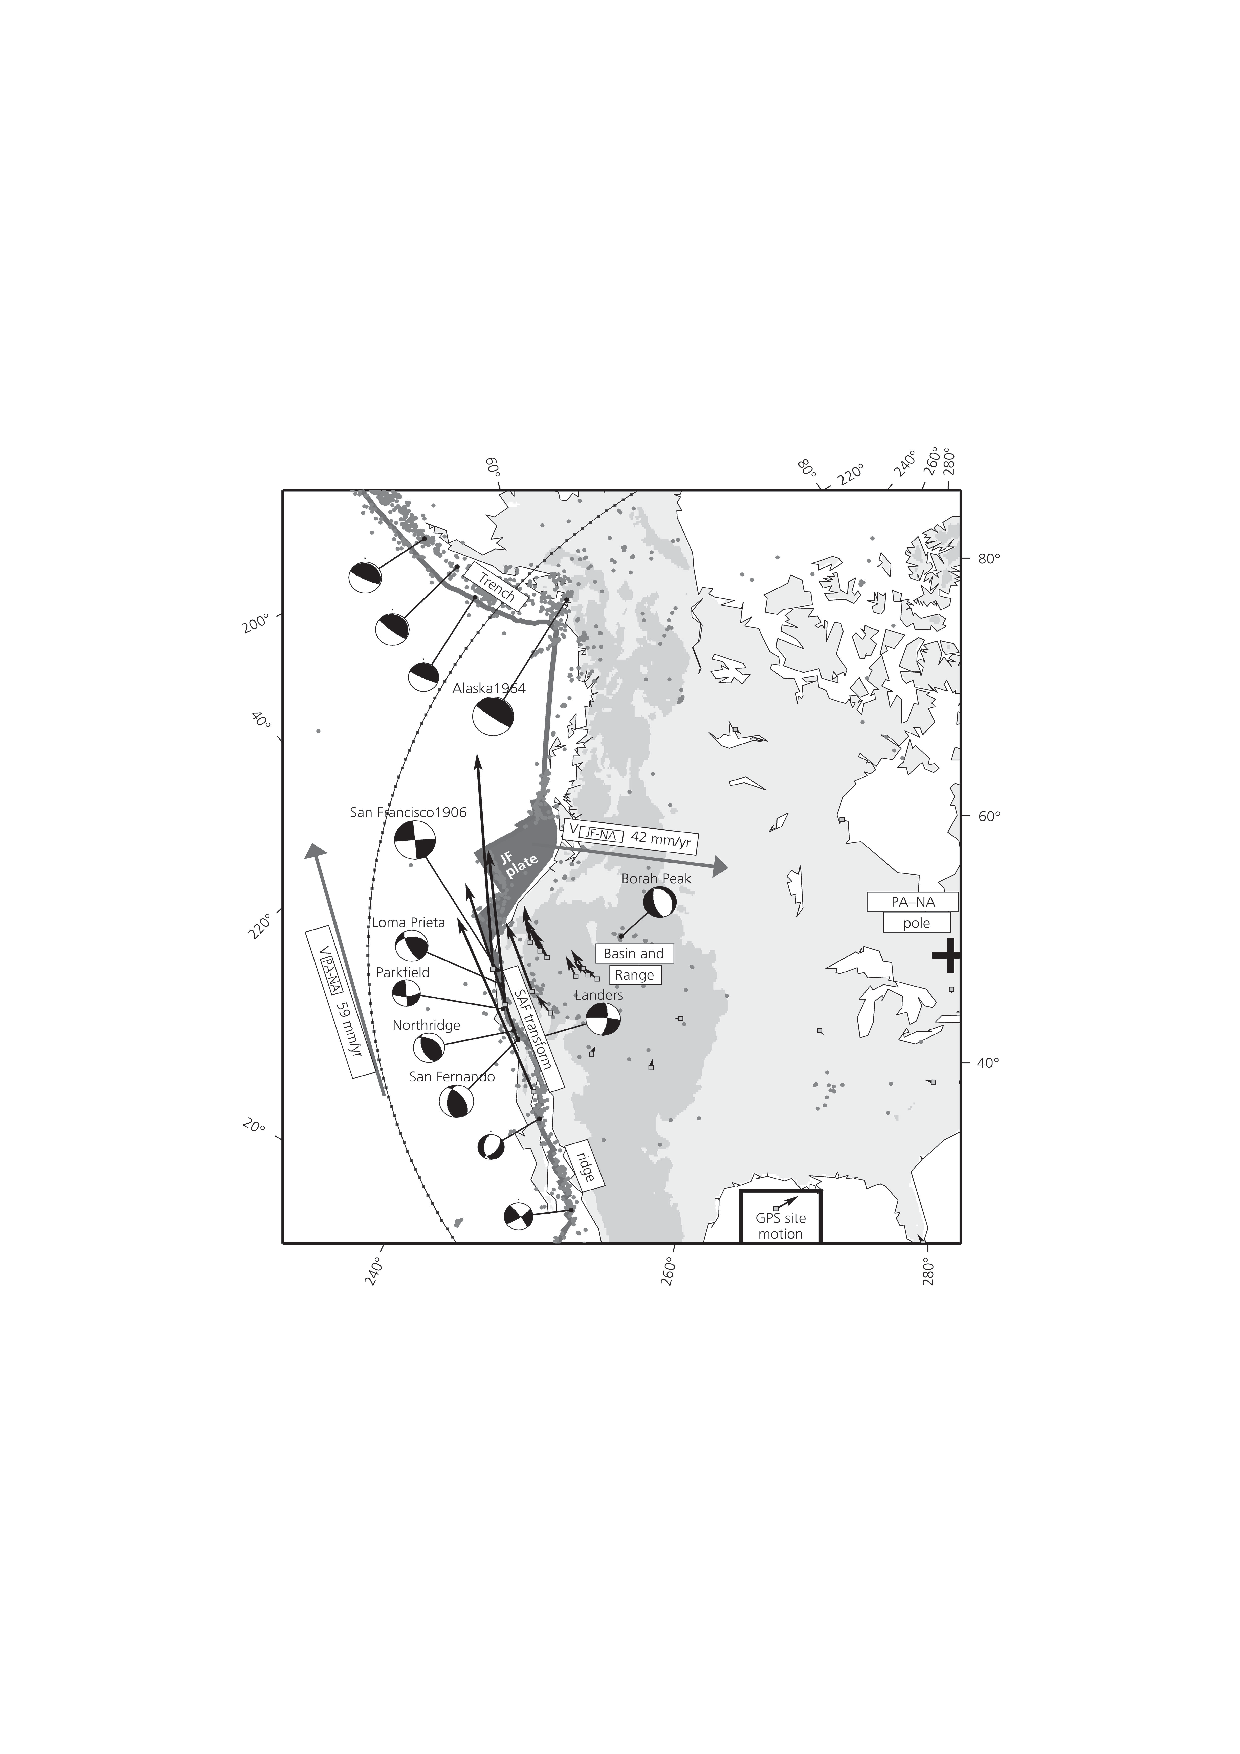
\includegraphics[trim = 0mm 70mm 0mm 70mm, clip,scale=0.6]{seismology/figures/map_with_FM.pdf}
    \caption{Map of North America with GPS movement (arrows) and earthquake
    (grey circles). Focal mechanisms indicate strike slip movements in
    California region, normal faults in Basin and Range area, and thrust
    movements in Alaska.  }
    \label{figure_map_FM}
\end{figure}

To construct a focal mechanism, only three parameters are required: the strike angle and dip angle of the fault, and the slip angle due to the earthquake displacement on the fault (see Figure~\ref{figure_fault_plan}). The strike angle $\Phi$ is defined as the angle in the plane of the earth's surface  measured clockwise from north to the fault direction ($0 \leqslant \Phi \leqslant 360$).  The dip angle $\delta$ gives the orientation of the fault plane with respect to the surface  ($0 \leqslant \delta \leqslant 90$). The final parameter is the slip angle $\lambda$ and give information about the movement : a slip angle of $\lambda$=0$^{\circ}$ indicates a \emph{left-lateral motion}; a slip angle of $\lambda$=180$^{\circ}$ shows a \emph{right-lateral motion}; a slip angle of $\lambda$=270$^{\circ}$ describes a \emph{normal faulting} ; finally a slip angle of $\lambda$=90$^{\circ}$ reveals a \emph{thrust faulting}. Sometimes, the dip angle is included between -180$^{\circ}$ to 180$^{\circ}$.
\begin{figure}[h!]
    \centering
    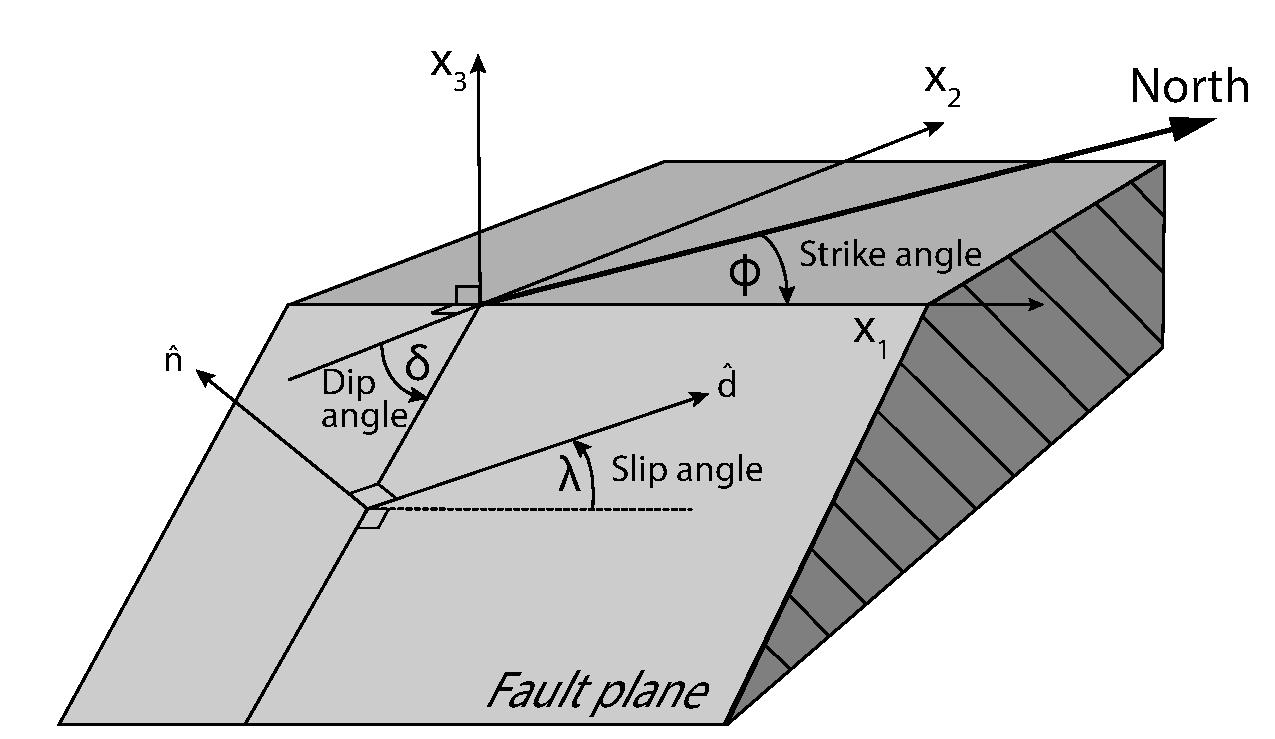
\includegraphics[trim = 0mm 140mm 0mm 0mm, clip,scale=0.5]{seismology/figures/figure_plan.pdf}
    \caption{Fault geometry used in earthquake studies.}
    \label{figure_fault_plan}
\end{figure}

Finally, we can construct the focal mechanism using stereonets and the procedure is shown for two examples in Figures~\ref{figure_FM_1} and \ref{figure_FM_2}.
\begin{figure}[h]
    \centering
    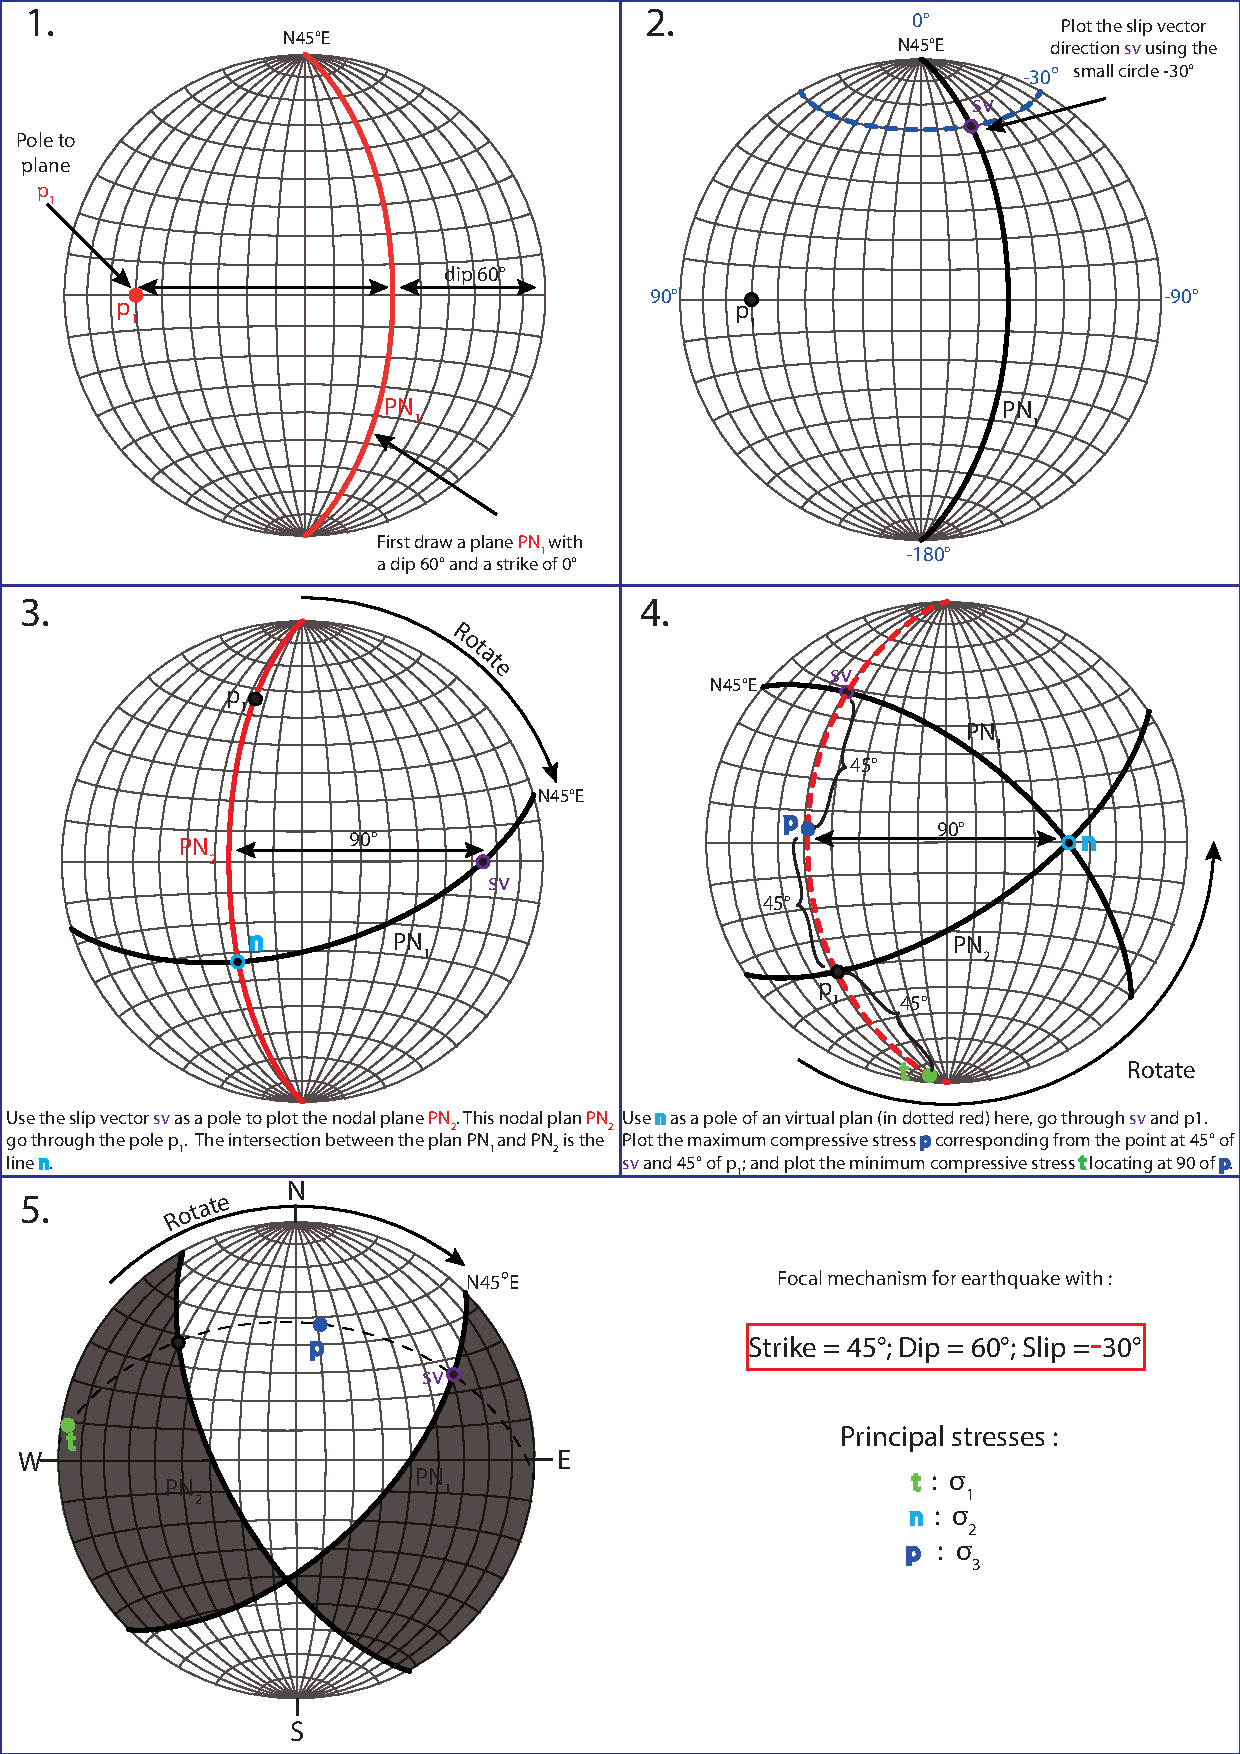
\includegraphics[trim = 0mm 0mm 0mm 0mm, clip,scale=0.6]{seismology/figures/stereonet_method_final_vertical.pdf}
    \caption{Focal mechanisms : example 1. This focal mechanism is constructed from the following parameters : $\Phi$=45$^{\circ}$; $\delta$=60$^{\circ}$; $\lambda$=-30$^{\circ}$. The 3 points $t$, $n$, and $p$ show the direction and dip of principal stresses $\sigma_1$, $\sigma_2$, and $\sigma_3$, respectively.}
    \label{figure_FM_1}
\end{figure}


\begin{figure}[h]
    \centering
    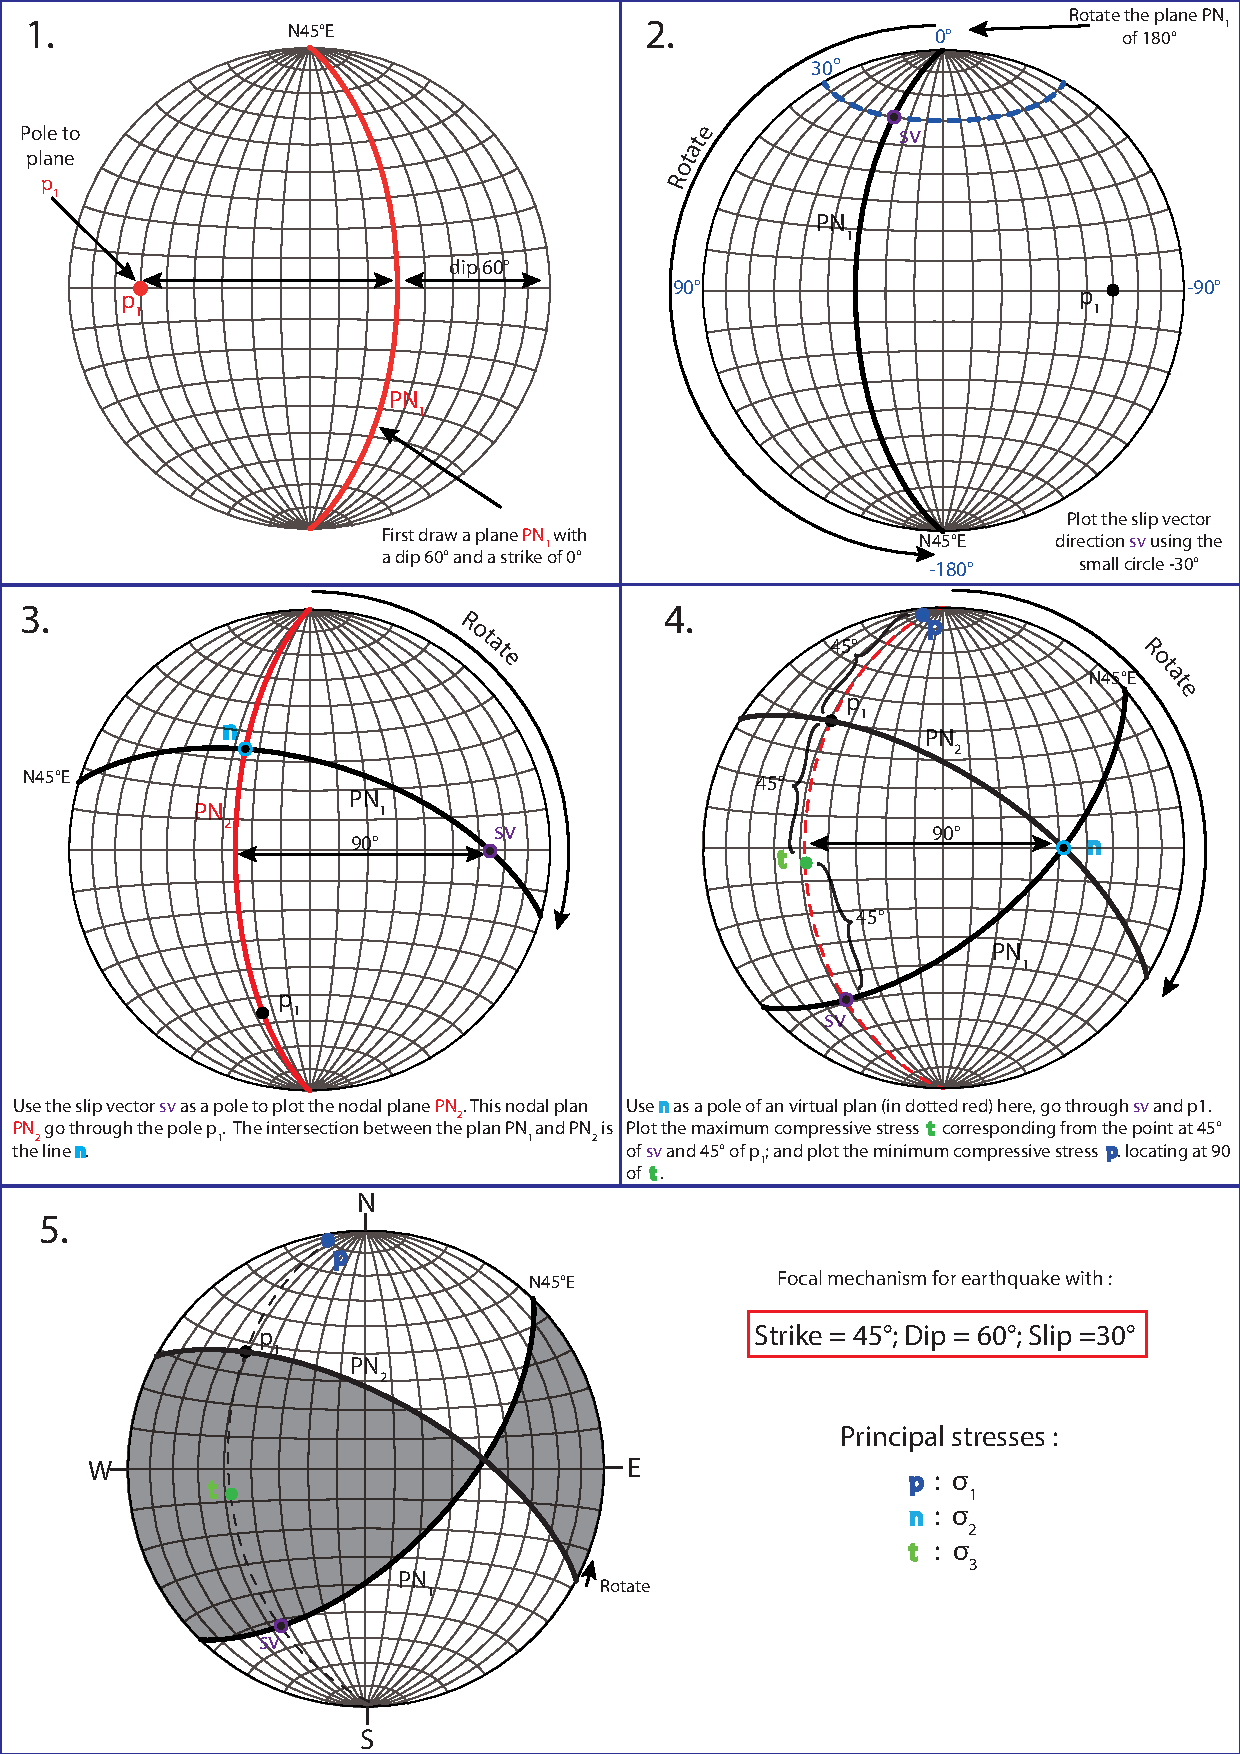
\includegraphics[trim = 0mm 0mm 0mm 0mm, clip,scale=0.6]{seismology/figures/stereonet_method_final_2_vertical.pdf}
    \caption{Focal mechanisms :  example 2. This focal mechanism is constructed from the following parameters : $\Phi$=45$^{\circ}$; $\delta$=60$^{\circ}$; $\lambda$=30$^{\circ}$.The 3 points $p$, $n$, and $t$ show the direction and dip of principal stresses $\sigma_1$, $\sigma_2$, $\sigma_3$ respectively.}
    \label{figure_FM_2}
\end{figure}


\subsection{Hudson diagram}
The Hudson diagram (a.k.a.\ source type plot, after Hudson, 1989) is useful for comparing the source types.  The center of the plot is a pure double couple (DC) solution.  Note this could be any double couple solution whether from a strike-slip, normal, reverse, or dip-slip fault.  The axis that falls between the $+$CLVD and $-$CLVD solutions represents no net volume change.  Above and below these zones, some volumetric change occurs during the rupture.
\begin{figure}[hbtp]
    \centering
    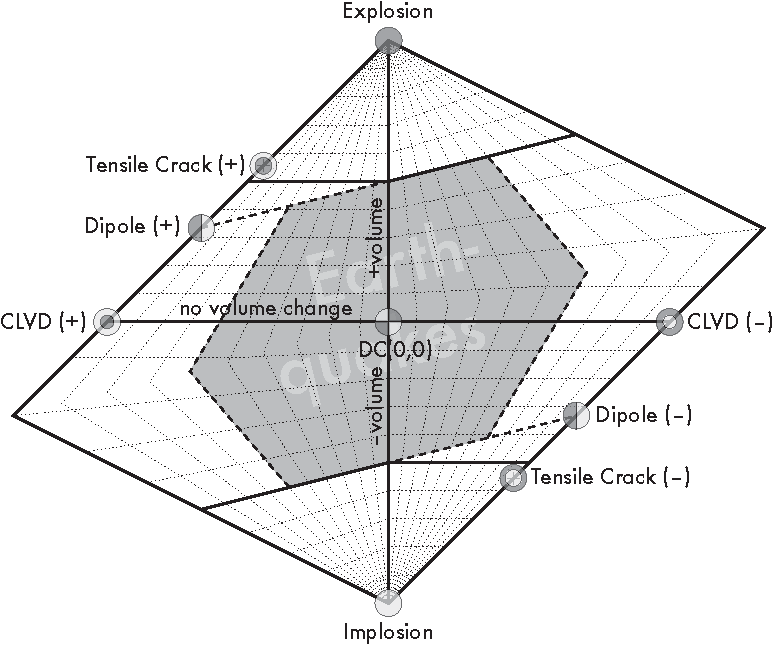
\includegraphics[]{seismology/figures/hudson_diagram2.pdf}
    \caption{Hudson diagram (source type plot) showing the distribution of possible source types.  DC is double couple (quadrupole) and CLVD is compensated linear vector dipole.  Focal mechanisms are plotted over ideal solutions to different pure source types.  Grey region is approximate region of most earthquakes.}
    \label{fig:hudson}
\end{figure}

Why might we find this useful?  For a collection of earthquakes and can help discriminate events based on multiple independent processes (Figure~\ref{fig:hudson}).  For example during volcanic eruptions, there may be several distinct episodes of magma injection and explosive volcanism.  These different source types may occur in spatially distinct regions or operate at different times.  Most earthquakes, but not all, fall within a defined region of the Hudson diagram centered about a pure double couple mechanism (grey region in Figure~\ref{fig:hudson}).

An example of a Hudson diagram for different source types is shown in Figure~\ref{fig:ford}.  Note the distinct differences in the locations of the source types.
\begin{figure}[hbtp]
    \centering
    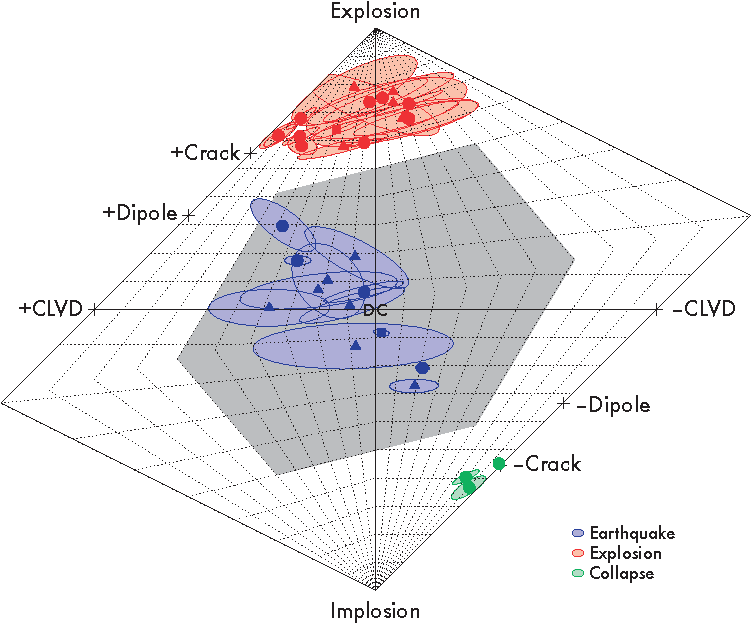
\includegraphics[]{seismology/figures/ford_etal2009_fig5.pdf}
    \caption{Source type plots for several earthquakes, nuclear explosions and
    mine collapses.  The shaded ovals represent 95\% confidence intervals.  After
    Ford et al. (2009).}
    \label{fig:ford}
\end{figure}


\section{Seismic Velocity}
The estimation of seismic velocity for minerals and rocks is discussed in Chapter~\ref{chap:physprop}.  Here we look at the effect of pressure and temperature on the seismic velocity for rocks instead of their consituent minerals.  Because models of seismic velocity estimates of the interior are more reliable than some other geophysical parameters made from surface observations, you will often find seismic velocity being used as a proxy used to estimate other physical properties.  Density is perhaps the most common of these so I include a little about the estimation of density from velocity in this section as well.

% P-T dependence
\subsection{$V_{P}$~Pressure~and~Temperature~Dependence}
Figure~\ref{fig:vpfit} illustrates the changes in seismic velocity as a function
of changes in temperature and pressure.
\begin{figure}[bthp]
    \centering
    \includegraphics[width=5.0in]{seismology/figures/gabbro.eps}
    \caption[Illustration of mathematical models used to predict seismic velocity.]{Mathematical preditions of the seismic velocity of gabbro.  P-wave velocity data of gabbro from \citet{Christensen&Mooney1995} (x's) are approximated using a pressure--temperature dependent model with (solid) and without (dashed) a crack closure term.  Each set of curves corresponds to data collected along at 20\degC\ or along a geothermal gradient of 8.9, 15.2, and 26.9\degC~km$^{-1}$.}
    \label{fig:vpfit}
\end{figure}
Each set of $V_{P}$ data corresponds to a different thermal gradient (curves labeled A (lowest) to D (highest)).  The constant temperature curve (A) shows an increase in velocity with pressure.  The other three (B--D) show a decrease in velocity with pressure because of the strong dependence of $V_{P}$ on temperature.

The effects of pressure and temperature are well known for a variety of rock types and tend to behave in a fairly predictable fashion.  Seismic P-wave velocity for a given rock can be expressed in terms of linear derivatives of pressure and temperature of the form
\begin{equation}
    V_{P}(P,T) = V^{\prime}_0
    + (T - T_{0})\left(\frac{\partial V_{P}}{\partial T}\right)_{P}
    + (P - P_{0})\left(\frac{\partial V_{P}}{\partial P}\right)_{T},
    \label{eq:pt}
\end{equation}
where $P_0$ and $T_0$ are the standard temperature and pressure conditions (STP) and $V^{\prime}_0$ is the p-wave velocity potential at STP.  The pressure and temperature deriviatives are measured in the labratory.  The pressure derivative for shallow crustal rocks is typically constant and independent of temperature at pressures up to 3 GPa \citep{Christensen&Mooney1995}.

The red curves in Figure~\ref{fig:vpfit} are computed using this model and generally fit the data well above 0.6~MPa or about 20~km depth.  So either this model is a poor approximation to the pressure affect or there are other influences on seismic velocity.  Since we know the seismic velocity of a rock is affected by several competing physical variables, including pressure, temperature, crack closure and mineral phase changes.  Since the data are most affected near the surface, it seems reasonable to assume fractures/cracks may have something to do with it.

% Crack closure
\subsection{Crack~Closure}
In the upper \SI{600}{MPa}, seismic velocities increase rapidly as a result of crack closure.  This increase is not described by Equation \ref{eq:pt}.  The effect of crack closure on seismic velocity can be generally expressed as
\begin{equation}
    V(P,T) = V^{\prime}(P,T) - f(P),
\end{equation}
where $V$ is the observed P-wave velocity and $V^{\prime}$ is the potential p-wave velocity absent the effects of cracks.  The function $f(P)$ represents the effect of crack closure on p-wave velocity.  To determine the nature of $f$, the contribution of the linear pressure derivative is removed (analagous to reduced temperature), leaving only the effects due to crack closure.  Three functional forms of $f$ were used to fit the crack effect: an inverse function, $f = a_{c}/P$; an exponential, $f = a_{c} \mbox{exp}(-P/P_{c})$; and an error function, $f = a_{c} \mbox{erfc}(P/P_{c})$.  The constant $a_{c}$ is a scaling factor and $P_{c}$ is the decay length.

An error function with a decay length $\sim$\SI{95}{MPa} best approximates the effect of crack closure on all rock samples.  At \SI{95}{MPa}, 84\% of the velocity increase due to crack closure has occurred.  Figure \ref{fig:crack}$a$ shows the a fit of the error function to a rock sample used in the analysis.  The error function describes the effect of crack closure quite well.  Unlike the decay depth, the scaling factor is much harder to determine.  Correlations between the scale factor (Figure \ref{fig:crack}$b$) and the velocity potential and density (Figure \ref{fig:crack}$c$) are very low ($r^2$ values 0.36 and 0.16).  Therefore, it appears that the scale factor is rock sample dependent and possibly the result of degree of fracturing and fracture orientations within a sample.  Once the scale factor for a particular rock has been determined, the revised function used to estimate seismic velocity becomes
\begin{equation}
    V_{P}(P,T) = V^{\prime}_{0} - a_{c} \mbox{erfc}(P/P_{c})
    + (T - T_{0})\left(\frac{\partial V_{P}}{\partial T}\right)_{P}
    + (P - P_{0})\left(\frac{\partial V_{P}}{\partial P}\right)_{T}.
    \label{eq:vp}
\end{equation}
\begin{figure}[tbhp]
    \centering
    \includegraphics{seismology/figures/crack.eps}
    \caption{Crack closure model.  $(a)$ Illustrates the best fitting crack closure model using an error function with $P_c = \SI{95}{MPa}$ (solid line).  Seismic velocity data from \citet{Kern_etal1999} are plotted as x's.  $(b)$ and $(c)$ displays the scaling factor as a function of potential seismic velocity and density.}
    \label{fig:crack}
\end{figure}
The velocity potential is determined by extrapolating the high pressure velocites unaffected by cracks to the surface.  A major difference between the data used to determine the $V_{P}$ relationship and model the the crack closure depth is the crack closure depth.

The fit of Equations~\ref{eq:pt} (dashed) and \ref{eq:vp} (solid) to the velocity data in Figure~\ref{fig:vpfit} shows the importance of a crack closure term below 600~MPa.  The fit of modeled crack effect on $V_{P}$ to the labratory data of gabbro shows a significant improvement over the purely $P$--$T$ model.

% Estimating Density
\subsection{Estimating~Densities}
The density increase with pressure can be described using a simple linear
relationship,
\begin{equation}
    \rho{_P} = \rho_{0} + (P - P_0)\left(\pdv{\rho}{P}\right)_T,
\end{equation}
where $\rho_{0}$ is surface density and $\left(\partial \rho/\partial P\right)$ is the pressure derivative of density at constant temperature.  The pressure derivative must be determined for each rock type based on experimental data.  A linear fit to the density data in \citet{Christensen&Mooney1995} yields a factor of 3 range of pressure derivatives from 15.6 to \SI{42}{kg.m^{-3}.MPa^{-1}} with a median of \SI{29.7}{kg.m^{-3}.MPa^{-1}}.  Temperature effects on density are not accounted for in the analysis by \citet{Christensen&Mooney1995} and are potentially larger than the effects of pressure.

An example of the fit to density is shown in Figure~\ref{fig:vprho}
\begin{figure}[tbhp]
    \centering
    \includegraphics{seismology/figures/velocity_to_density.eps}
    \caption{Velocity to density models fit to a number of rocks types.  Two models are shown for igneous and metamrophic rocks (red) by {\citet{Christensen&Mooney1995}}. The \citet{Barton1986} model was developed for sedimentary rocks (grey).  The yellow points are monomineralic rocks not included in fit.}
    \label{fig:vprho}
\end{figure}

The prefered model used to estimate the density from seismic velocity is given by the linear seismic velocity to density relationship \citep{Christensen&Mooney1995} given by
\begin{equation}
  \label{eq:cmlinear}
  \rho = a + b V_{P},
\end{equation}
where $a$ and $b$ are empirically derived coefficients.  \textit{Christensen and Mooney} published coefficients to the linear $V_{P}$--$\rho$ equation for a temperature of \si{309}{\degC}\ and pressures equivalent to 5 to 50~km in increments of 5~km.  Therefore, it is necessary to determine the coefficients to all other crustal $P$--$T$ conditions for this study.  Having developed a method to extend density and seismic velocity to a greater range of $P$--$T$ conditions, the empirical coefficients are determined using a linear least-squares inversion to polymineralic rock types at the range of crustal pressures ranging from 0 to 2.6~GPa and temperatures from 20 to \si{1300}{\degC}.  Monominearlic rock types are excluded from determining the coefficients in the linear relationship as they tend to have high velocities with low density or vice versa. Figure~\ref{fig:empconst}
$a$ and $b$ contour the linear coefficients ($a$ and $b$ from Equation~\ref{eq:cmlinear}) for an extended range of pressure and temperature conditions
for the depth and temperature.
\begin{figure}[tbhp]
    \centering
    \includegraphics{seismology/figures/CM95linear.eps}
    \caption[Empirical coefficients for the linear $V_{P}$--$\rho$ conversion by \citet{Christensen&Mooney1995}.]{Empirical coefficients for the linear $V_{P}$--$\rho$ conversion by \citet{Christensen&Mooney1995} are gridded for range of possible $P$--$T$ conditions.}
    \label{fig:empconst}
\end{figure}
%\FloatBarrier

\ntextbox{Stress Fields Across Regimes: Static, Diffusive, and Wave Behavior}{
    With so many geophysical fields bridging the various PDE realms, you may be asking yourself whether elastic fields---seismic fields are elastic waves---admit similar steady-state and diffusive behaviors.  The short answer is no, not directly; but the longer answer is that elastic stress fields do exhibit elliptic, parabolic and hyperbolic regimes, but these operate on different spatial and temporal scales and are not observed in the same way as classical geophysical fields, as summarized below.

    Stress and strain in the solid Earth are governed by the same underlying mechanical framework, but admit distinct mathematical regimes depending on the relative importance of inertia and dissipation. These regimes operate on different spatial and temporal scales and are sampled by different observational approaches.

    \begin{enumerate}
        \item \textbf{Static (Elastic Equilibrium)}

        In the absence of inertia, long-term tectonic stresses satisfy the equations of static elasticity:
        \[
            \div{\bm{\sigma}} + \vb{f} = 0, \quad \bm{\sigma} = \vb{C} \colon \bm{\varepsilon}, \quad \bm{\varepsilon} = \tfrac{1}{2}(\grad{\vb{u}} + \grad{\vb{u}^\mathsf{T}}),
        \]
        where $\vb{f}$ is the body force per unit volume, and $\vb{C}$ is the fourth-order elastic stiffness tensor.

        This system is elliptic and defines a boundary-value problem for displacement and stress. Static stress fields reflect present-day plate boundary forces and loads, modified by elastic structure and heterogeneity. Although well-posed mathematically, stress is not directly observable at depth; surface measurements are sparse, load-contaminated, and path-dependent.

        \item \textbf{Diffusive (Stress Relaxation)}

        When dissipation is introduced through viscoelastic or poroelastic behavior, stress evolves diffusively at long times:
        \[
            \pdv{\bm{\sigma}}{t} = D_\sigma \,\laplacian{\bm{\sigma}}, \quad D_\sigma \sim \frac{\mu}{\eta},
        \]
        where $D_{\sigma}$ is the effective stress diffusivity.

        This parabolic regime governs postseismic deformation and long-term tectonic relaxation, primarily within the ductile lower crust and upper mantle. The characteristic timescale is the Maxwell relaxation time, $\tau_M = \eta/\mu$, where $\eta$ is the effective viscosity and $\mu$ is the shear modulus.

        which typically ranges from decades to thousands of years depending on rheology. In the continental crust, effective relaxation times are commonly $10^1--10^3$ years, while in the upper mantle they may be shorter where viscosities are lower. This diffusive regime underlies postseismic deformation, where stress perturbations introduced by earthquakes relax through viscoelastic flow and poroelastic pressure diffusion. Observational access to this regime is indirect, relying on geodetic measurements (e.g., GPS, InSAR) rather than traditional geophysical field observations.

        \item \textbf{Wave Propagation (Seismology)}

        Including inertia yields the elastic wave equation:
        \[
            \rho \, \pdv[2]{\vb{u}}{t} = \div{(\vb{C} \colon \grad \vb{u})},
        \]
        which is hyperbolic and supports propagating seismic waves. This regime samples transient stress disturbances rather than the background stress field. Wave propagation does not relax to a steady-state or diffusive limit; once energy propagates away, the field vanishes.
    \end{enumerate}

    \noindent\textbf{Interpretation and Observability}\\
    Although static and diffusive stress fields are physically real and mathematically well defined, they do not constitute classical geophysical field methods because stress is not directly observable at depth. Consequently, these regimes are treated primarily within geodesy and tectonics, while seismology focuses on the hyperbolic, wave-propagation regime where signals are directly measurable.  This distinction mirrors that between elliptic, parabolic, and hyperbolic governing equations encountered elsewhere in geophysics, but highlights that the existence of a governing PDE does not guarantee a usable geophysical observable.
}{aside}


\nocite{Fowler1990}
\nocite{Lowrie1997}
\nocite{Schey1997}

\bibliographystyle{elsarticle-harv}
\bibliography{ref}
